%% ============================================================================
%% Journal of Information Security and Applications (JISA) submission.
%% Prepared with Elsevier's elsarticle class.
%%
%% Compile options:
%%   Author-facing draft: default (single-column, 12pt, line numbers, todos).
%%   Camera-ready:        remove [preprint,review,authoryear,12pt] switches
%%                        below, add [final,3p,times,twocolumn] to switch to
%%                        the journal's production style, and change
%%                        \usepackage{todonotes} to \usepackage[disable]{todonotes}.
%% ============================================================================
% \documentclass[preprint, review, authoryear, 12pt]{elsarticle}
\documentclass[final,3p,times,twocolumn]{elsarticle}

\journal{Journal of Information Security and Applications}

% Author–date citations (JISA style)
\usepackage[authoryear]{natbib}
% Line numbers for reviewer PDF (comment out for camera-ready)
%\usepackage{lineno}
%\linenumbers
\usepackage{comment}
% Standard packages used across tables, figures, algorithms, and the pipeline diagram
\usepackage{amsmath, amssymb, amsfonts}
\usepackage{booktabs}
\usepackage{array}
\usepackage{multirow}
\usepackage{tikz}
\usepackage{xcolor}
\usepackage{enumitem}
\usetikzlibrary{
	shapes.geometric,
	arrows.meta,
	positioning,
	fit,
	backgrounds,
	calc
}
\usepackage{float}
\usepackage{capt-of}
\usepackage[ruled, linesnumbered]{algorithm2e}
\usepackage{graphicx}
\usepackage{orcidlink}
\usepackage{scalerel,stackengine}
\def\apeqA{\SavedStyle\sim}
\def\apeq{\setstackgap{L}{\dimexpr.5pt+1.5\LMpt}\ensurestackMath{%
  \ThisStyle{\mathrel{\Centerstack{{\apeqA} {\apeqA}}}}}}

% Review-mode annotations. Switch to \usepackage[disable]{todonotes} for the
% camera-ready version to suppress the reviewer margin notes without deleting
% them from the source.
\usepackage[ textsize=footnotesize, textwidth=1.8cm]{todonotes}


\begin{document}
	\begin{frontmatter}
		\title{Strengthening User Privacy through AI-Driven Assurance Quantification
		and International Standards Alignment}

		\author[ku]{Jordan (Jay) Bell Compaan\corref{cor1}}\ead{k2119852@kingston.ac.uk}
		\cortext[cor1]{Corresponding author}

		\author[ku]{Razi Arshad}\ead{R.Arshad@kingston.ac.uk}

		\affiliation[ku]{organization={Kingston University London}, addressline={55--59 Penrhyn Road}, city={Kingston upon Thames}, postcode={KT1 2EE}, country={United Kingdom}}

		% ==========================================================================
		% Abstract
		% ==========================================================================
		\begin{abstract}
NLP systems classify privacy-policy clauses accurately but their predictions are rarely 
linked to auditable evidence from privacy regulations and standards. We propose 
\textbf{PrERT-CNM} (\textbf{P}rivacy B\textbf{ERT} with \textbf{C}ontextual \textbf{N}
eural \textbf{M}emory), a framework coupling a fine-tuned privacy-domain transformer, a 
retrieval memory over a harmonised regulatory-control catalogue, and a Bayesian 
aggregation layer. The CNM uses a ChromaDB-backed dense-vector index and a gated auxiliary 
logit head, leaving the PrivBERT clause input unchanged. This design provides a trace 
from each prediction to retrieved GDPR, ISO/IEC, and NIST Privacy framework controls.
            
An ablation over $k \in \{0, 1, 3, 5, 10\}$ identifies $k=10$ as the headline retrieval-
enabled configuration. On the policy-partitioned OPP-115 test set ($n=2{,}472$ clauses), 
it achieves an accuracy of $96.16\%$ ($0.9616$), macro-F1 of $0.8826$, and a 
configuration-weighted primary evidence score of $0.9412$. The retrieval-disabled 
configuration achieved an accuracy of $95.91\%$ ($0.9591$) and a macro-F1 score of 
$0.8857$. Thus, the retrieval-enabled model does not improve overall macro-F1, but 
provides standards-linked traceability while retaining broadly comparable predictive 
performance. The $k=3$ configuration exhibits a larger reduction in macro-F1 to $0.8467$, 
showing that performance preservation is not guaranteed for every retrieval budget. The 
headline model's recorded test expected calibration error is $0.0212$. Independent 
validation of clause-to-control retrieval and of the relationship between the aggregated 
evidence score and expert assessments remains necessary.


            
		\end{abstract}
\begin{comment}
       \onecolumn
        \begin{highlights}
            \begin{itemize}
                \item PrERT\-CNM: PrivBERT \+ retrieval memory \+ Bayesian aggregation for privacy assurance
                \item Harmonised 683-control catalogue: GDPR, 8 ISO/IEC standards, NIST Privacy Framework
                \item Gated auxiliary-head CNM ablated over top-$k$ retrieval budget on OPP-115
                \item Cluster-bootstrap 95\% CI [0.870, 0.922] on macro-F1 with policy-level split
                \item Every posterior traceable to source clause and originating regulatory provision
            \end{itemize}
        \end{highlights}
\end{comment}

		\begin{keyword}
			privacy assurance quantification \sep natural language processing \sep BERT
			\sep retrieval-augmented memory \sep Bayesian inference \sep GDPR \sep ISO/IEC
			controls \sep NIST Privacy Framework
		\end{keyword}
	\end{frontmatter}

	% ============================================================================
	% General response to reviewer
	% ============================================================================

    % ============================================================================

    
    \section{Introduction}
	\label{sec:intro}
    Online services rely on privacy policies as the principal, and often only, instrument through which individuals are informed of how their personal data are collected, processed, and shared. Such documents are typically long, legally dense, and difficult to compare across services, which limits the ability of users to give informed consent and to make meaningful choices	between providers. In parallel, organisations must satisfy overlapping obligations under the EU General Data Protection Regulation (GDPR) \citep{gdpr2016}, the ISO/IEC 27000 and 29100 families of information-security and privacy standards \citep{iso27001_2022,iso27002_2022,iso29100_2011}, and the NIST Privacy Framework \citep{nist_pf_2020}. These regulatory instruments articulate normative requirements but do not, by themselves, define the	quantitative, observable evidence needed to measure how well a specific policy addresses them.
    
	\subsection{Current State of the Art and Its Limits}
	\label{sec:sota} Three complementary research strands have advanced automated privacy-policy analysis to its current state. First, corpus construction and clause classification:	the OPP-115 corpus \citep{wilson2016opp115} established a benchmark of 115 manually annotated privacy policies and remains the canonical supervised anchor; hierarchical neural classifiers \citep{harkous2018polisis} and mobile-app compliance systems \citep{zimmeck2019maps} have scaled category prediction to large	volumes of text, and privacy-domain transformers \citep{srinath2021privaseer,muralitharan2024privacybertlstm} have raised clause-classification accuracy substantially. Second, standards-to-metrics operationalisation: legal ontologies such as PrOnto \citep{palmirani2018pronto} and P2Onto \citep{novikova2025privacyrisks} encode GDPR concepts in a shared vocabulary; NIST PRAM \citep{brooks2017nistpram} formalises analyst-driven privacy risk assessment; and controls-mapping efforts translate regulatory text into structured control catalogues. Third, quantitative aggregation: Bayesian and ontology-based methods aggregate evidence into numerical scores \citep{novikova2025privacyrisks,oetzel2014pia}.	What none of these strands provides, however, is a single pipeline that starts from natural-language policy text and produces standards-linked, multi-level assessments with calibrated uncertainty. The interpretation strand stops at category labels; the operationalisation strand stops at conceptual mapping; and the aggregation strand assumes structured inputs. This paper is motivated by, and addresses, the gaps left between these three strands. 
    
	\subsection{Three Gaps in Existing Research}
	\paragraph{Gap 1: from clause labels to standards-linked evidence}
    
	\emph{What existing work does:} clause classifiers assign OPP-115 or similar categorical labels to policy sentences with high accuracy \citep{harkous2018polisis,srinath2021privaseer,muralitharan2024privacybertlstm}.
    
	\emph{What is missing:} no widely adopted pipeline links those labels to the specific regulatory provisions that a clause satisfies or fails to disclose. 
    
    \emph{Why it matters:} without such a link, a category label such as ``First-Party 	Collection/Use'' cannot be used to answer the operational question, ``does this policy provide the evidence that GDPR Article 5 requires?''
    
	\paragraph{Gap 2: from normative text to quantitative indicators.}
    
	\emph{What existing work does:} standards \citep{gdpr2016,iso27001_2022,nist_pf_2020} and legal ontologies \citep{palmirani2018pronto} articulate obligations. 
    
    \emph{What	is missing:} they do not define the quantitative, observable evidence needed to measure them at scale on natural-language text. 
    
    \emph{Why it matters:} without observable indicators, ``appropriate technical and organisational measures'' cannot be audited by any procedure other than expert reading.
	
    \paragraph{Gap 3: from noisy clause-level evidence to a defensible summary.}
	
    \emph{What existing work does:} weighted-score \citep{novikova2025privacyrisks} and likelihood--impact \citep{brooks2017nistpram} approaches aggregate evidence into a single number.
    
    \emph{What is missing:} calibrated uncertainty,	per-level decomposition, and traceability from the summary back to individual policy sentences.
    
    \emph{Why it matters:} a scalar score without uncertainty misrepresents its own reliability, particularly when the underlying evidence is sparse for a given policy or level.

	\subsection{Construct Definition and Scope}
	\label{sec:construct} 
    

This study distinguishes four constructs. \emph{Clause-level classification} denotes assignment of a policy clause to the user, system, or organisation level. \emph{Standards-linked traceability} denotes retrieval of named regulatory controls that can be inspected alongside a prediction. \emph{Policy-disclosed control coverage} denotes the breadth and adequacy with which a policy addresses applicable controls. \emph{Legal compliance} denotes whether an organisation's actual practices satisfy applicable law. The present evaluation directly tests the first construct and demonstrates the technical production of the second. It does not independently validate the third or fourth.

The Bayesian output reported in this paper is therefore defined narrowly as \emph{confidence-weighted level-evidence posterior}. For a policy $\mathcal{P}$ and level $\ell\in\{\text{user},\text{system},\text{organisation}\}$, the posterior summaries the confidence attached to clauses predicted at level $\ell$. Under Equation~\ref{eq:bayes-update}, each such clause contributes $w_i c_i$ to $\alpha^{(\ell)}$ and $w_i(1-c_i)$ to $\beta^{(\ell)}$. Consequently, the posterior is not mathematically equivalent to a simple unweighted mean of evidence-count-dependent posterior distribution. Nevertheless, it remains principally a transformation of classifier confidence.

In particular, the current update does not reward coverage of additional unique controls, distinguish repeated evidence for one control from evidence spanning several controls, or estimate whether a reviewed control is adequately satisfied. A policy containing many confidently classified clauses can therefore receive a high level-evidence posterior while covering only a narrow subset of the applicable control catalogue. Retrieved control identifiers are retained as an auditable trace, but they do not currently enter the likelihood term.

Accordingly, the posterior must not be interpreted as the probability that a policy complies with GDPR, ISO/IEC, or NIST requirements, nor as a validated measure of organisational privacy risk. It is an uncertainty-aware summary of classification evidence whose relationship to expert-assessed disclosed assurance remains to be established. A control-coverage-aware formulation and independent expert validation are identified as required extensions.
    

	\subsection{Framework and Research Questions}
	The paper proposes \textbf{PrERT-CNM} (\emph{Privacy BERT with Contextual Neural Memory}), a framework that couples (i) a fine-tuned privacy-domain transformer classifier, (ii) a retrieval-augmented Contextual Neural Memory over a harmonised standards catalogue, and (iii) a Bayesian aggregation layer that returns per-level assurance posteriors with 95\% credible intervals. The framework follows a design-science methodology \citep{hevner2004design}: an artefact is designed, built, and evaluated iteratively on the OPP-115 corpus \citep{wilson2016opp115,opp115_dataset}.

To the best of the authors' knowledge, and consistent with the most recent survey of privacy quantification \citep{arshad2024characterisation}, no prior work simultaneously (i) extracts a harmonised, machine-readable control catalogue from the GDPR, the ISO/IEC 27000/29100 standards families and the NIST Privacy Framework, (ii) fine-tunes a privacy-specific transformer classifier and integrates its clause probabilities into a level-specific Bayesian model whose priors are elicited from standards expectations, and (iii) reports per-regulation verdicts whose supporting clauses are individually citable. The recent P2Onto approach \citep{novikova2025privacyrisks} is the closest antecedent but operates on a small manual sample of three policies and does not report calibrated uncertainty. Existing transformer approaches \citep{srinath2021privaseer,muralitharan2024privacybertlstm} stop at clause labels. The empirical evaluation answers four research questions:
	\begin{itemize}
		\item \textbf{RQ1.} How accurately can privacy-policy clauses be classified into user-, system-, and organisation-level obligations under strict policy-level data separation?

		\item \textbf{RQ2.} Can heterogeneous regulatory provisions be represented in a shared machine-readable catalogue and used to produce inspectable clause-to-control retrieval traces?
        
		\item \textbf{RQ3.} How does confidence-weighted Bayesian aggregation summarise clause-level classification evidence across the user, system, and organisation levels, and how sensitive is  that summary to evidence sparsity, duplication, calibration, and prior selection?

		\item \textbf{RQ4.} How robust are the resulting scores to class imbalance, clause duplication, and Bayesian prior selection?
	\end{itemize}

RQ2 evaluates implementation and trace production rather than independently validated retrieval accuracy. Claims about clause-to-control correctness remain conditional until the Stage-B human evaluation described in Section~\ref{sec:phase1} is complete.

Each research question is mapped to specific experiments in Section~\ref{sec:methodology} and answered in Section~\ref{sec:results}.

	\subsection{Scientific Contributions}
	The scientific contributions of this research are as follows:
	\begin{enumerate}
		\item A machine-readable catalogue that harmonises 683 extracted controls from GDPR, eight ISO/IEC standards, and the NIST Privacy Framework while retaining source identifiers and regulatory provenance.

		\item A gated auxiliary-head Contextual Neural Memory that attaches inspectable standards-control retrieval traces to clause predictions. The retrieval-enabled headline configuration retains broadly comparable macro-F1 to the retrieval-disabled PrivBERT configuration, but is not presented as an overall classification improvement.

        \item A Bayesian evidence-aggregation layer that converts clause-level classification confidence into per-level posterior distributions and retains the contributing clauses and retrieved controls. These outputs are treated as confidence-weighted evidence summaries rather than independently validated probabilities of control coverage or legal compliance.

	\end{enumerate}

Implementation features: the acceptance-check tooling, synthetic policy/schema fixtures, the Gradio web demonstrator, and the variant-tracked evaluation stack are engineering deliverables and are documented alongside the released code and model checkpoint \citep{prertcnm_github,prertcnm_huggingface}.

	\paragraph{Paper organisation.}
Section~\ref{sec:literature} critically reviews related work. Section~\ref{sec:framework} describes the PrERT-CNM framework, including the CNM module. Section~\ref{sec:methodology} details the methodology. Section~\ref{sec:results} reports the experiments. Section~\ref{sec:discussion} discusses interpretation, limitations, ethics, and future work. Section~\ref{sec:conclusion} concludes.

	% ==========================================================
	\section{Related Work}
	\label{sec:literature} This section reviews four research strands and, for
	each strand, critically identifies (i) what existing work achieves, (ii) its
	limitations, and (iii) the unresolved gap that PrERT-CNM addresses. The
	comparative comparison against the closest prior systems is presented in Table~\ref{tab:litcompare}.
	
	\subsection{AI for Privacy-Policy Analysis}
	\emph{Achievement.} Automated privacy-policy analysis has progressed through three
	overlapping generations: annotated corpora with classical machine learning
	\citep{wilson2016opp115,sathyendra2017optout,poplavska2020gdprmap};
	hierarchical neural classifiers and mobile-app compliance systems \citep{harkous2018polisis,zimmeck2019maps};
	and privacy-domain transformers \citep{devlin2019bert,srinath2021privaseer,muralitharan2024privacybertlstm}.
	Parallel work on legal NLP has explored rationale extraction and retrieval-augmented
	question answering \citep{chalkidis2022legalnlp,ravichander2019qa}. \emph{Limitation.}
	Across all three generations, systems output categorical labels or per-clause
	probabilities. They do not link those probabilities to specific regulatory provisions,
	they do not aggregate them into level-specific summaries, and they rarely accompany
	their outputs with uncertainty. \emph{Unresolved gap.} The step from category labels
	to standards-linked, calibrated, multi-level assessments remains open. PrERT-CNM
	addresses this step through the CNM module and the Bayesian aggregation layer.

	\subsection{Privacy Quantification and Breach Analytics}
	\emph{Achievement.} Privacy risk has been formalised along several dimensions.
	Solove's taxonomy \citep{solove2006taxonomy} organises harms conceptually.
	Likelihood--impact methodologies operationalise privacy impact assessment \citep{brooks2017nistpram,oetzel2014pia}.
	Threat-modelling frameworks such as LINDDUN \citep{deng2011linddun} enumerate
	privacy threat categories. Ontology-based methods such as P2Onto \citep{novikova2025privacyrisks}
	derive numerical scores from the presence of critical data types and coverage
	of purposes, legal bases, and opt-out options. Empirical breach corpora \citep{enisa_tl_2024,prc_breaches}
	supply frequency and severity evidence for the harms dimension. \emph{Limitation.}
	Quantitative work typically operates at a single level of abstraction, treats likelihood
	and impact as scalar analyst inputs, and rarely connects the resulting score
	to specific standards obligations \citep{arshad2024characterisation}. Ontology-based
	scoring \citep{novikova2025privacyrisks} works on a manual sample of three policies
	and does not report calibrated uncertainty. Breach corpora are decoupled from
	policy text. \emph{Unresolved gap.} A concrete mechanism for aggregating
	clause-level policy evidence into per-level, standards-linked posterior estimates
	with credible intervals. PrERT-CNM addresses this through the retrieval-augmented
	CNM (which links clauses to specific provisions) and Beta--Bernoulli aggregation
	(which produces credible intervals).

	\subsection{Standards and Regulatory Frameworks}
	\emph{Achievement.} Control-based frameworks provide auditable structure. The GDPR
	\citep{gdpr2016} establishes principles (Article~5), security obligations (Article~32),
	and breach notification (Article~33). The ISO/IEC family \citep{iso27001_2022,iso27002_2022,iso27005_2022,iso27018_2019,iso27701_2019,iso29100_2011,iso29151_2017,iso15944_12_2020},
	the NIST Privacy Framework \citep{nist_pf_2020}, the NIST AI Risk Management Framework
	\citep{nist_aiRMF_2023}, and the EU AI Act \citep{eu_ai_act_2024} together
	codify obligations spanning security, privacy, and AI governance. Legal ontologies
	\citep{palmirani2018pronto,novikova2025privacyrisks} and machine-readable-policy
	languages \citep{cranor2002p3p,ashley2003epal,gerl2018lpl,pardo2019pilot} formalise
	these obligations. Automated GDPR-compliance systems \citep{amaral2021gdprnn} apply
	rule-based or shallow-neural techniques to check specific articles. \emph{Limitation.}
	Standards leave measurement to implementers, ontologies focus on
	representation rather than automated measurement, and policy languages require
	policy authors to write in the formal language rather than in natural English.
	Automated compliance work targets specific articles or DPAs rather than the
	natural-language policies presented to end users. \emph{Unresolved gap.} A
	pipeline that operates directly on the natural-language policy text and links
	each clause to the relevant provision across three standards families
	simultaneously. PrERT-CNM addresses this by combining the harmonised control catalogue
	with the CNM retriever and the Bayesian layer.

	\subsection{Probabilistic Risk Modelling}

    
	\emph{Achievement.} 
    Probabilistic graphical models \citep{pearl1988probabilistic,koller2009pgm}
	provide the general formalism for reasoning under partial evidence; Bayesian
	text classification \citep{domingos1997optimality} demonstrates conjugate updates
	on categorical evidence; and Beta--Bernoulli belief updating \citep{gelman2013bayesian}
	is the textbook choice for evidence that takes the form of independent
	Bernoulli-like signals with an unknown rate. 
    
    \emph{Limitation.} The
	independence assumption is violated when clauses within the same policy reuse
	phrasing, and softmax classifier probabilities are not, in general, probabilities
	that a regulatory control is satisfied. 

    \emph{Position adopted in this Study.} 
    The resulting posterior is interpreted only as a confidence-weighted level evidence summary. It is not 
    interpreted as a posterior probability that a regulatory control is satisfied. Duplicate sensitivity is examined 
    separately, while calibration must be estimated on the validation partition applied before final aggregation. 
    A stronger assurance formulation would use independently evaluated clause-to-control relevance 
    probabilities, unique-control coverage, and evidence adequacy as explicit likelihood components.
    
    \emph{Unresolved gap.} A formulation that
	(i) is theoretically justified as an assurance measure rather than a compliance
	guarantee, (ii) is empirically calibrated at the per-class level, and (iii) accommodates
	within-policy dependence at evaluation time. Section~\ref{sec:phase3} states
	the theoretical justification, Section~\ref{sec:calibration} reports per-class
	calibration, and Section~\ref{sec:calibration} handles within-policy
	dependence via policy-level cluster bootstrapping.

	\subsection{Synthesis and Positioning}
	Table~\ref{tab:litcompare} compares representative prior systems against PrERT-CNM
	on the dimensions most relevant to standards-linked assurance quantification. The
	comparison is presented descriptively rather than as Yes/No columns, so that
	PrERT-CNM is judged on the same attributes as the systems it extends.
    \onecolumn
    \begin{table}
		[ht]
		\centering
		\caption{Descriptive comparison of representative privacy-analysis and
		privacy-quantification approaches against PrERT-CNM.}
		\label{tab:litcompare} \scriptsize
		\setlength{\tabcolsep}{5pt}
		\renewcommand{\arraystretch}{1}
		
        \resizebox{\columnwidth}{!}{
        \begin{tabular}{@{}>{\raggedright\arraybackslash}p{0.11\linewidth}>{\raggedright\arraybackslash}p{0.11\linewidth}>{\raggedright\arraybackslash}p{0.11\linewidth}>{\raggedright\arraybackslash}p{0.11\linewidth}>{\raggedright\arraybackslash}p{0.11\linewidth}>{\raggedright\arraybackslash}p{0.11\linewidth}>{\raggedright\arraybackslash}p{0.11\linewidth}>{\raggedright\arraybackslash}p{0.11\linewidth}>{\raggedright\arraybackslash}p{0.11\linewidth}@{}}
			\toprule \textbf{Study}                                  & \textbf{Dataset}    & \textbf{NLP method}                          & \textbf{Granularity}& \textbf{Regulatory mapping}& \textbf{Score definition}                    & \textbf{Uncertainty}& \textbf{Traceability}& \textbf{External val.}                                  \\
			\midrule OPP-115 \citep{wilson2016opp115}                & OPP-115             & Manual annot.                                & Segment                          & None                              & ---                                          & ---                                                 & ---                                          & Inter-annot. agreement                                  \\
			Polisis \citep{harkous2018polisis}                       & OPP-115             & Hierarchical CNN                             & Segment                          & None                              & ---                                          & Softmax only                                        & Category label                               & Crowd study                                             \\
			MAPS \citep{zimmeck2019maps}                             & APP-350             & NLP + static                                 & App                              & Mobile privacy law                & Rule violation                               & ---                                                 & Rule ID                                      & Manual audit                                            \\
			PrivacyBERT-LSTM \citep{muralitharan2024privacybertlstm} & Custom              & BERT + LSTM                                  & Sentence                         & None                              & ---                                          & Softmax only                                        & ---                                          & ---                                                     \\
			PrivaSeer / PrivBERT \citep{srinath2021privaseer}        & PrivaSeer           & Domain-pretrained BERT                       & Corpus / clause                  & None                              & ---                                          & ---                                                 & ---                                          & Downstream tasks                                        \\
			P2Onto \citep{novikova2025privacyrisks}                  & OPP-115 (3 pol.)    & Ontology + rules                             & Data-practice                    & GDPR concepts                     & Weighted PD types                            & ---                                                 & Ontology class                               & Expert scoring (n=7)                                    \\
			NIST PRAM \citep{brooks2017nistpram}                     & N/A (questionnaire) & ---                                          & System                           & NIST PF                           & Likelihood$\times$impact& Analyst judgement                                   & Risk register                                & ---                                                     \\
			Arshad and Asghar \citep{arshad2024characterisation}     & --- (survey)        & ---                                          & Conceptual                       & Cross-framework                   & Multi-dim. (concept)                         & ---                                                 & ---                                          & ---                                                     \\
			\textbf{PrERT-CNM (this work)}                           & \textbf{OPP-115}    & \textbf{PrivBERT + CNM retrieval + Bayesian} & \textbf{Clause + policy + level} & \textbf{GDPR, 8~ISO/IEC, NIST~PF} & \textbf{Confidence-weighted level-evidence summary} & \textbf{95\%~credible intervals; cluster bootstrap} & \textbf{Clause $\to$ control $\to$ standard} & \textbf{Policy-level split; case study; expert planned} \\
			\bottomrule
		\end{tabular}}
	\end{table}
    \twocolumn
    % ==========================================================
	\section{Proposed AI-Driven Assurance Quantification Framework}
	\label{sec:framework} The proposed framework, PrERT-CNM, is implemented as a
	reproducible four-phase pipeline. Each phase emits versioned artefacts (JSON
	Lines records and manifests) that serve as verified inputs to the next. Figure~\ref{fig:pipeline}
	summarises the project workflow at the phase level, and Figure~\ref{fig:inference}
	shows the run-time inference path for a single policy.

	\begin{center}
		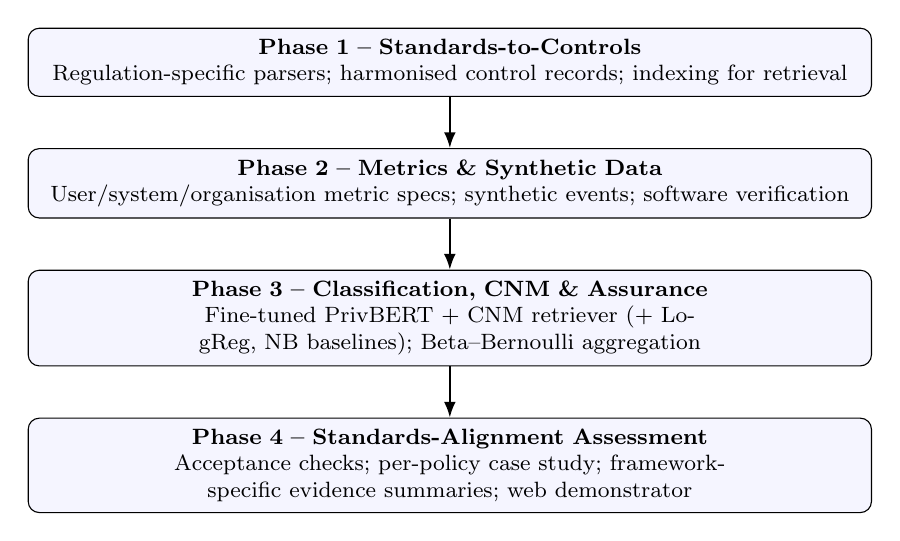
\begin{tikzpicture}[
			node distance=6.5mm,
			box/.style={draw, rounded corners, align=center, inner sep=4pt, text width=0.86\columnwidth, font=\footnotesize, fill=blue!4},
			arr/.style={-{Latex[length=2mm]}, thick}
		]
			\node[box] (p1)
			{\textbf{Phase 1 -- Standards-to-Controls}\\ Regulation-specific parsers; harmonised control records; indexing for retrieval};
			\node[box, below=of p1] (p2) {\textbf{Phase 2 -- Metrics \& Synthetic Data}\\ User/system/organisation metric specs; synthetic events; software verification};
			\node[box, below=of p2] (p3)
			{\textbf{Phase 3 -- Classification, CNM \& Assurance}\\ Fine-tuned PrivBERT + CNM retriever (+ LogReg, NB baselines); Beta--Bernoulli aggregation};
			\node[box, below=of p3] (p4) {\textbf{Phase 4 -- Standards-Alignment Assessment}\\ Acceptance checks; per-policy case study; framework-specific evidence summaries; web demonstrator};
			\draw[arr] (p1) -- (p2); \draw[arr] (p2) -- (p3); \draw[arr] (p3) -- (p4);
		\end{tikzpicture}
		\captionof{figure}{Project workflow.} \label{fig:pipeline}
	\end{center}


    \begin{figure}[h]
        \centering
        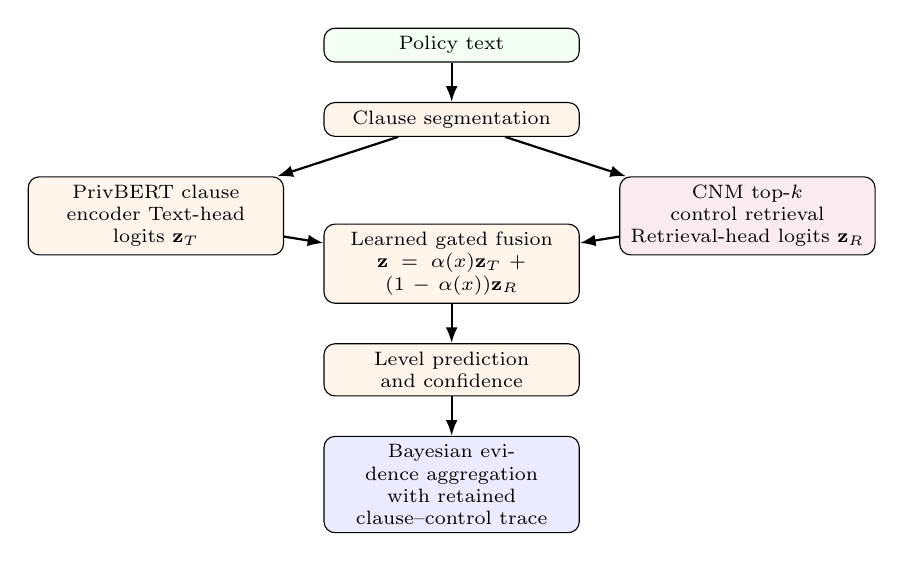
\begin{tikzpicture}[
            node distance=5mm and 5mm,
            box/.style={
                draw,
                rounded corners,
                align=center,
                inner sep=3pt,
                text width=0.25\columnwidth,
                font=\scriptsize
            },
            input/.style={box,fill=green!5},
            process/.style={box,fill=orange!8},
            memory/.style={box,fill=purple!8},
            output/.style={box,fill=blue!8},
            arr/.style={-{Latex[length=2mm]},thick}
        ]
            \node[input] (policy) {Policy text};
            \node[process,below=of policy] (segment) {Clause segmentation};
    
            \node[process,below left=of segment] (texthead)
            {PrivBERT clause\\encoder Text-head\\logits $\mathbf{z}_{T}$};
    
            \node[memory,below right=of segment] (retriever)
            {CNM top-$k$\\control retrieval\\Retrieval-head logits
            $\mathbf{z}_{R}$};
    
            \node[process,below=11mm of segment] (gate)
            {Learned gated fusion\\
            $\mathbf{z}=\alpha(x)\mathbf{z}_{T}
            +(1-\alpha(x))\mathbf{z}_{R}$};
    
            \node[process,below=of gate] (prediction)
            {Level prediction and confidence};
    
            \node[output,below=of prediction] (aggregation)
            {Bayesian evidence aggregation\\
            with retained clause--control trace};
    
            \draw[arr] (policy) -- (segment);
            \draw[arr] (segment) -- (texthead);
            \draw[arr] (segment) -- (retriever);
            \draw[arr] (texthead) -- (gate);
            \draw[arr] (retriever) -- (gate);
            \draw[arr] (gate) -- (prediction);
            \draw[arr] (prediction) -- (aggregation);
        \end{tikzpicture}
    
        \caption{Inference path for one policy clause. The clause is supplied
        unchanged to the PrivBERT text head and independently embedded for
        top-$k$ control retrieval. Text and retrieval logits are combined by the
        learned gate before classification. The Bayesian layer aggregates the
        resulting confidence while retaining the retrieved-control trace.}
        \label{fig:inference}
    \end{figure}

	A unifying abstraction is the three-level privacy taxonomy given in Table~\ref{tab:labelspace},
	which maps every OPP-115 data-practice category onto the \texttt{user},
	\texttt{system}, or \texttt{organisation} level. The taxonomy defines the
	classifier label space, the granularity of the metric specifications, and the
	structure of the Bayesian posteriors.

	\begin{table}[!h]
		\centering
		\caption{Complete mapping of the ten OPP-115 data-practice categories onto
		the three-level PrERT-CNM taxonomy.}
		\label{tab:labelspace}
		The mapping is an analyst-defined abstraction for this study, not a
		validated ontology. User-level categories describe choices and rights
		exercised by the data subject; system-level categories describe
		technical or interaction mechanisms; the remaining categories describe
		controller or processor practices and are assigned to the organisation
		level. The fixed user $\succ$ system $\succ$ organisation precedence
		preserves the more specific subject-facing interpretation when a clause
		has multiple OPP-115 labels. No independent expert review or
		alternative-mapping sensitivity analysis was present in the freeze, so
		taxonomy validity remains a limitation.
        \footnotesize
		\begin{tabular}{@{}p{0.28\columnwidth} p{0.62\columnwidth}@{}}
			\toprule \textbf{PrERT-CNM level} & \textbf{OPP-115 categories mapped to this level}                                                                                       \\
			\midrule \texttt{user}            & User Choice/Control; User Access, Edit and Deletion                                                                                    \\
			\texttt{system}                   & Data Security; Do Not Track                                                                                                            \\
			\texttt{organisation}             & First-Party Collection/Use; Third-Party Sharing/Collection; Data Retention; International and Specific Audiences; Policy Change; Other \\
			\bottomrule
		\end{tabular}
	\end{table}
    
	\subsection{Phase 1: Standards-to-Controls Extraction}
	\label{sec:phase1} Phase~1 converts heterogeneous regulatory documents into a harmonised,
	machine-readable control catalogue. A \emph{control} is defined here as the
	smallest requirement-bearing unit that (i) originates from a single top-level
	clause, article, or subcategory of a source document, (ii) states a specific,
	testable expectation on a data controller or processor, and (iii) can be independently
	referred to by a normalised identifier. When a top-level provision contains
	multiple sub-requirements (for example, GDPR Article~5 lists six principles),
	each sub-requirement is retained as a separate control if it is testable in
	isolation and would otherwise be lost in aggregation. 

	Rather than a single generic parser, the framework employs \emph{regulation-specific}
	parsers that respect each document's structure: GDPR articles, ISO/IEC clauses
	and bullet hierarchies, and NIST Privacy Framework subcategories are each handled
	by a dedicated extractor. Each extracted control is stored as a record with a
	normalised identifier (for example, \texttt{gdpr::Article\_32}), its hierarchical
	path, the source text, and a parser-confidence score. Control text is then
	segmented and indexed for retrieval by the CNM module.

	\paragraph{Overlap and merging.}
	Two controls from different standards frequently express overlapping requirements
	(e.g., GDPR Art.~32 on ``appropriate technical and organisational measures'' and
	ISO/IEC 27002:2022 clause 8.24 on cryptographic controls both articulate technical-security
	expectations). PrERT-CNM does not merge such controls: each control retains
	its source identifier, and the CNM retriever surfaces all overlapping controls
	for a clause whose embedding lies within threshold. This preserves per-standard
	traceability, at the cost of some redundancy in the retrieved context. A cross-standard
	\emph{crosswalk} field is attached to each control record, listing sibling
	controls in other standards; the crosswalk is used only to report per-regulation
	evidence summaries in Phase~4. 
	
    \paragraph{Extraction statistics.}
	Table~\ref{tab:phase1-stats} summarises extraction statistics per source. The
	released repository \citep{prertcnm_github} contains the full manifest with parser-confidence
	distributions for each control.

	\begin{table}[h]
		\centering
		\caption{Phase~1 extraction statistics per regulatory source.}
		\label{tab:phase1-stats} \footnotesize
		\setlength{\tabcolsep}{5pt}
    
		\resizebox{\columnwidth}{!}{
        \begin{tabular}{@{}l r r r@{}}
			\toprule \textbf{Source}            & \textbf{Provisions}  & \textbf{Controls}  & \textbf{Retained}    \\
			                                    & \textbf{processed}   & \textbf{extracted} & \textbf{after norm.} \\
			\midrule GDPR (Regulation 2016/679) & 99 articles          & 187                & 187                  \\
			ISO/IEC 27001:2022                  & 10 clauses + Annex~A & 93                 & 93                   \\
			ISO/IEC 27002:2022                  & 4 domains            & 93                 & 93                   \\
			ISO/IEC 27005:2022                  & 10 clauses           & 41                 & 41                   \\
			ISO/IEC 27018:2019                  & 18 clauses           & 30                 & 30                   \\
			ISO/IEC 27701:2019                  & 5 clauses            & 84                 & 84                   \\
			ISO/IEC 29100:2011                  & 5 clauses            & 11                 & 11                   \\
			ISO/IEC 29151:2017                  & 18 clauses           & 27                 & 27                   \\
			ISO/IEC 15944-12:2020               & 8 clauses            & 17                 & 17                   \\
			NIST Privacy Framework 1.0          & 5 functions          & 100                & 100                  \\
			\midrule \textbf{Total}             & ---                  & \textbf{683}       & \textbf{683}         \\
			\bottomrule
		\end{tabular}
        }
	\end{table}

	\paragraph{Two-stage validation protocol.}
	Extraction and retrieval require separate validation. \emph{Stage A: parser
	correctness.} A stratified sample of 200 controls (20 per source, drawn uniformly
	across the parser-confidence range) is manually inspected; a control is judged
	correct if its identifier, hierarchical path, and source text match the corresponding
	provision in the source document. \emph{Stage B: clause-to-control mapping accuracy.}
	A stratified sample of 200 policy clauses drawn from the OPP-115 training partition
	(proportional to level distribution) is labelled by two independent annotators
	with the correct control identifier for each clause; inter-annotator agreement
	is reported (Cohen's $\kappa$), and the CNM retriever's top-$k$ output is scored
	against this reference by recall@$k$ for $k \in \{1, 3, 5\}$. Stage~B is intentionally
	distinct from Stage~A because a correctly extracted provision does not guarantee
	that a clause has been correctly linked to it.

	The reported freeze contains only a preliminary Stage A inspection: 57 of 60
	sampled controls were judged correct on first inspection (95.0\%). This result
	is a feasibility check rather than the prespecified 200-control estimate of
	parser correctness, and it is not used to claim that the full catalogue has
	been independently validated.

	Stage B was specified as a separate human evaluation but was not completed in
	the reported artefacts. The intended sample is 200 clauses drawn from the
	OPP-115 training partition, stratified by the three-level label distribution
	and sampled without replacement at the policy level. Two annotators, blinded
	to the CNM output, independently assign zero or more candidate control IDs
	from the frozen 683-control catalogue to each clause and record an explicit
	``no applicable control'' outcome when appropriate. Disagreements are
	adjudicated only after the independent labels are locked. Agreement is to be
	reported using Cohen's $\kappa$ on the primary control assignment, with
	``no applicable control'' treated as a valid category. For each clause, the
	frozen $k=10$ CNM ranking is then compared with the adjudicated reference and
	reported as Recall@$k$ for $k \in \{1,3,5,10\}$, with bootstrap confidence
	intervals clustered by policy. The annotator form, catalogue hash, sampled
	clause IDs, adjudicated labels, and scoring script should be archived with
	the resulting metrics to make the evaluation auditable.

	Because the Stage B annotations and scores were not present at the freeze,
	Cohen's $\kappa$ and Recall@$1$, Recall@$3$, Recall@$5$, and Recall@$10$ are
	not reported here. The evidence therefore supports the narrower claim that
	the system generates inspectable clause-to-control traces; it does not yet
	establish their retrieval accuracy or validate the correctness of individual
	mappings. Independent Stage A completion and Stage B human evaluation remain
	prerequisites for a stronger traceability claim.
  

	\subsection{Phase 2: Metrics, Synthetic Data, and Software Verification}
	\label{sec:phase2} Phase~2 translates the Phase~1 controls into metric
	specifications. Table~\ref{tab:metrics} lists the metrics used at each level.
	Each metric specifies its scoring formula, evidence fields, standards-control
	identifiers, normalisation rule, missing-data treatment, and direction.

	\begin{table*}
		[h]
		\centering
		\caption{Metric specifications used at each level of the PrERT-CNM taxonomy.
		Missing evidence is recorded as \texttt{null} and the metric's contribution
		is set to its prior expectation, so that a policy is not penalised for silence
		unless silence is itself a control failure.}
		\label{tab:metrics}
		The seven Phase~2 metrics are specification and software-verification
		artefacts in the reported freeze; they are not additional likelihood
		terms in Equation~\ref{eq:bayes-update}. The final posterior is updated
		from the predicted level, classifier confidence, prior, and optional
		deduplication weight only. Consequently, these rows document intended
		evidence fields and control provenance but do not establish control
		coverage or alter the reported posterior.
        
        \scriptsize
		\setlength{\tabcolsep}{5pt}
		\resizebox{\textwidth}{!}{
        \begin{tabular}{@{}ll>{\raggedright\arraybackslash}p{0.15\linewidth}>{\raggedright\arraybackslash}p{0.09\linewidth}>{\raggedright\arraybackslash}p{0.09\linewidth}>{\raggedright\arraybackslash}p{0.09\linewidth}l@{}}
			\toprule \textbf{Level} & \textbf{Metric ID}              & \textbf{Scoring formula}                                                                 & \textbf{Evidence fields}                                         & \textbf{Standards source}                  & \textbf{Normalisation} & \textbf{Direction}          \\
			\midrule user           & \texttt{consent\_control}       & Fraction of clauses describing opt-in/opt-out choices, weighted by classifier confidence & \texttt{clause\_id}, \texttt{confidence}, \texttt{choice\_type}  & GDPR~Art.~6; ISO/IEC~29100                 & Scaled to [0,1]        & Higher = stronger assurance \\
			user                    & \texttt{user\_access\_deletion} & Fraction of clauses describing subject rights (access, correct, delete)                  & \texttt{clause\_id}, \texttt{confidence}, \texttt{right\_type}   & GDPR~Arts.~15--17; ISO/IEC~27701           & Scaled to [0,1]        & Higher = stronger assurance \\
			system                  & \texttt{security\_controls}     & Fraction of clauses describing technical security measures                               & \texttt{clause\_id}, \texttt{confidence}, \texttt{control\_type} & GDPR~Art.~32; ISO/IEC~27002; NIST~PF PR.PT & Scaled to [0,1]        & Higher = stronger assurance \\
			system                  & \texttt{tracking\_controls}     & Fraction of clauses describing tracking, Do Not Track, or cookie preferences             & \texttt{clause\_id}, \texttt{confidence}                         & ISO/IEC~29100; NIST~PF CT.PO               & Scaled to [0,1]        & Higher = stronger assurance \\
			organisation            & \texttt{collection\_use}        & Fraction of clauses declaring lawful specific purposes of collection                     & \texttt{clause\_id}, \texttt{confidence}, \texttt{purpose}       & GDPR~Art.~5; ISO/IEC~27701                 & Scaled to [0,1]        & Higher = stronger assurance \\
			organisation            & \texttt{third\_party\_sharing}  & Fraction of clauses declaring third-party recipients and legal basis                     & \texttt{clause\_id}, \texttt{confidence}, \texttt{recipient}     & GDPR~Arts.~26,~44; ISO/IEC~27018           & Scaled to [0,1]        & Higher = stronger assurance \\
			organisation            & \texttt{retention\_governance}  & Fraction of clauses describing retention periods and governance                          & \texttt{clause\_id}, \texttt{confidence}, \texttt{duration}      & GDPR~Art.~5(1)(e); ISO/IEC~27701           & Scaled to [0,1]        & Higher = stronger assurance \\
			\bottomrule
		\end{tabular}
        }
	\end{table*}

	\paragraph{Software-verification role of the synthetic data.}
	Phase~2 generates synthetic observations across three scenarios (\emph{normal},
	\emph{stressed}, \emph{adversarial}) with a fixed random seed. In each scenario
	500 observations are drawn per metric. The \emph{normal} scenario samples check
	counts from $\text{Poisson}(\lambda{=}20)$, failure counts from
	$\text{Binomial}(n{=}\text{checks}, p{=}0.05)$, and observed confidence from $\text{Beta}
	(8, 2)$; the \emph{stressed} scenario raises the failure rate to $p{=}0.20$ and
	shifts observed confidence to $\text{Beta}(5, 5)$; the \emph{adversarial} scenario
	applies $p{=}0.50$, injects missing fields on 30\% of observations, and
	samples confidence from $\text{Beta}(2, 8)$. \emph{Scope.} These synthetic
	scenarios are used \emph{only} for software verification: they confirm that
	the aggregation code preserves the theoretically expected ordering \emph{normal}
	$\prec$ \emph{stressed} $\prec$ \emph{adversarial} (mean scoring residual
	$0.06$, $0.27$, $0.55$) and that missing-evidence handling widens credible intervals
	as intended. They do not appear in any empirical result: real-policy validation
	is performed exclusively on OPP-115 (Section~\ref{sec:results}) and independent
	expert validation is planned as future work. 
	\subsection{Phase 3: Contextual Neural Memory, Classification, and Bayesian Aggregation}
	\label{sec:phase3}
	The analytical core of PrERT-CNM has three coupled components: a \emph{Contextual
	Neural Memory} that retrieves relevant regulatory controls for each policy
	clause (Section~\ref{sec:cnm}), a fine-tuned \emph{PrivBERT classifier} that
	assigns clauses to levels using the retrieved context, and a \emph{Bayesian
	aggregation layer} that produces per-level assurance posteriors. The novel components
	are (i) the CNM retriever, (ii) its coupling with the classifier at inference
	time, and (iii) the Bayesian layer whose priors are elicited from standards expectations
	and whose per-level output is auditable back to individual sentences.

	\subsubsection{Contextual Neural Memory}
	\label{sec:cnm} The CNM is a gated, auxiliary-head retrieval component over
	the harmonised standards catalogue. In contrast to a text-concatenation design
	that prepends retrieved control text to the tokeniser input, the CNM leaves
	the clause encoder input unchanged and introduces retrieval as a \emph{parallel}
	logit stream combined with the text-classifier stream through a learned scalar
	gate. This design decision follows from a preliminary experiment (Section~\ref{sec:cnm-preliminary})
	in which naive input-concatenation retrieval-augmentation collapsed minority-class
	discrimination on the OPP-115 training distribution; the auxiliary-head design
	was introduced specifically to protect minority-class geometry while retaining
	retrieval traceability.

	Formally, given clause $x$, tokeniser $T$, PrivBERT encoder $E_{\theta}$, memory
	index $\mathcal{M}= \{(v_{i}, e_{i})\}_{i=1}^{|\mathcal{M}|}$ where $v_{i}$ is
	the control record and $e_{i} \in \mathbb{R}^{d}$ is its fixed dense embedding
	under sentence encoder $\phi$, and label alphabet
	$\mathcal{Y}= \{y_{1}, \ldots, y_{C}\}$:

	\begin{align}
		h(x)              & = E_{\theta}(T(x))_{[\text{CLS}]}\in \mathbb{R}^{H}, \label{eq:cnm-encoder}                                              \\
		R_{k}(x)          & = \operatorname*{arg\,top-}k_{i}\; \cos\!\bigl(\phi(x),\, e_{i}\bigr), \label{eq:cnm-retriever}                          \\
		\text{logits}_{T} & = W_{T}\, h(x) + b_{T}, \qquad W_{T} \in \mathbb{R}^{C \times H}, \label{eq:cnm-text-head}                               \\
		\text{logits}_{R} & = \sum_{j=1}^{k}\operatorname{softmax}\!\bigl(\mathbf{s}(x)/\tau\bigr)_{j} \cdot L[r_{j}], \label{eq:cnm-retrieval-head} \\
		\alpha(x)         & = \sigma\!\bigl(w_{g}^{\top}\, \tanh(W_{g}\, h(x)) + b_{g}\bigr) \in (0,1), \label{eq:cnm-gate}                          \\
		\text{logits}(x)  & = \alpha(x)\, \text{logits}_{T} + \bigl(1 - \alpha(x)\bigr) \text{logits}_{R}, \label{eq:cnm-combined}
	\end{align}

	where $L \in \mathbb{R}^{|\mathcal{M}| \times C}$ is a matrix of learned per-control
	label logits, $\mathbf{s}(x) \in \mathbb{R}^{k}$ contains the cosine
	similarities of the top-$k$ retrieved controls, $\tau$ is a retrieval-attention
	temperature, and $\alpha(x)$ is the per-example gate that chooses how much of
	the class decision comes from the clause representation itself (text head)
	versus from the retrieved standards evidence (retrieval head). When $k = 0$,
	the retrieval branch is disabled ($\alpha \equiv 1$) and the model reduces
	exactly to the plain-PrivBERT baseline. The retrieval head is initialised at $L
	\equiv 0$ and the gate at $b_{g} = +2$ (giving $\alpha(x) \approx 0.88$ at
		step $0$), so the retrieval branch is initially zero-valued and the initial
		logit stream is a scaled text-only stream. This initialization property does
		not guarantee the behaviour of the trained model; the ablation includes a
		material degradation at $k=3$.

	\paragraph{Retrieval consistency loss.}
	The per-control logit matrix $L$ receives its training signal from two sources:
	(i) the main task cross-entropy on Equation~\ref{eq:cnm-combined}, backpropagated
	through the retrieval-head branch, and (ii) an auxiliary consistency term
	$\mathcal{L}_{\text{cons}}$ that pulls each row $L[j]$ towards the empirical
	class distribution of clauses that retrieve control $j$ in their top-$k$:
	\begin{equation}
		\mathcal{L}_{\text{cons}}= \frac{\lambda}{|\mathcal{B}_{R}|}\sum_{j \in
		\mathcal{B}_R}\mathrm{KL}\!\Bigl(\hat{P}(y \mid j) \;\Big\Vert\; \mathrm{softmax}
		(L[j])\Bigr), \label{eq:cnm-consistency}
	\end{equation}
	where $\mathcal{B}_{R}$ is the set of unique controls retrieved by the current
	batch, $\hat{P}(y \mid j)$ is a smoothed empirical class distribution computed
	once from the training set, and $\lambda$ is a small mixing weight ($\lambda =
	0.1$
	in the reported runs). This term prevents the retrieval head from collapsing
	to a class prior and gives each retrieved control an auditable, per-class contribution.

	\paragraph{Implementation.}
	The memory index is built once from the Phase~1 harmonised controls by the
	\texttt{prert-cnmv2 build-chroma} entry point of the accompanying software release~\citep{prertcnm_github}.
	The embedding function $\phi$ is the pretrained sentence-transformers checkpoint
	\texttt{all-MiniLM-L6-v2}, producing $d = 384$-dimensional $\ell_{2}$-normalised
	vectors; cosine similarity is therefore an inner product on the normalised
	matrix, and top-$k$ selection uses \texttt{numpy.argpartition} followed by a
	stable descending sort for deterministic tie-breaking. The catalogue is persisted
	in a ChromaDB collection with a SHA-256 corpus hash to detect stale rebuilds,
	and mirrored to an in-memory \texttt{float32} matrix at fit time so the training
	loop performs batched top-$k$ retrieval without per-step Chroma queries.
	Training is orchestrated through a Hugging Face \texttt{Trainer} subclass whose
	\texttt{compute\_loss} adds Equation~\ref{eq:cnm-consistency} to the class-weighted
	focal loss described in Section~\ref{sec:classifier}. The full model surface (text
	head, retrieval head control logits, gate MLP, encoder backbone) is trained
	end-to-end at learning rate $5 \times 10^{-5}$ for three epochs. A warm-up option
	freezes the retrieval head and the gate for the first epoch, letting the text
	head converge to the baseline decision boundary before the retrieval head
	starts contributing gradient; this option is enabled in the freeze reported below.

	\paragraph{Interpretability and traceability.}
	The retrieval-augmented forward pass exposes three interpretable signals per
	prediction. (i) The identifiers of the top-$k$ retrieved controls $\{v_{r_1}, \ldots
	, v_{r_k}\}$ and their similarity scores are attached to every clause prediction
	and propagate into the per-regulation evidence summaries emitted in Phase~4. (ii)
	The gate value $\alpha(x) \in (0,1)$ reveals, per clause, how much the model trusted
	retrieval-based evidence versus the clause representation alone;
	$\alpha \to 1$ indicates the text head sufficed, $\alpha \to 0$ indicates retrieval
	dominated. (iii) The per-control label matrix $L$ can be inspected offline as
	a $|\mathcal{M}| \times C$ table showing, for each retrieved control, its
	learned contribution to each class. The sparse memory ($|\mathcal{M}| = 683$
	harmonised controls, plus derived indicators expanding the addressable retrieval
	surface to $956$ entries) is versioned alongside the Phase~1 catalogue so
	every retrieved item is a named regulatory control or a derived indicator that
	can be inspected directly.
	The released freeze does not report gate-value summaries by class or retrieval
	budget. Accordingly, the architecture exposes $\alpha(x)$ as an inspectable
	signal, but the current evidence does not establish how much the trained model
	uses the retrieval stream in aggregate.
	\subsubsection{Clause Classification}
	\label{sec:classifier} The primary classifier fine-tunes the PrivBERT
	checkpoint \texttt{mukund/privbert} \citep{srinath2021privaseer} using Hugging
	Face Transformers \citep{wolf2020transformers} and PyTorch \citep{paszke2019pytorch}.
	To counter the pronounced class imbalance of the corpus, training uses a class-weighted
	focal-loss objective \citep{lin2017focal}:
	\begin{equation}
		\mathcal{L}_{\text{FL}}(p_{t}) = -\alpha_{c} \,(1 - p_{t})^{\gamma}\, \log p_{t}
		, \label{eq:focal}
	\end{equation}
	where $p_{t}$ is the softmax probability of the ground-truth class, $\alpha_{c}$
	is the class weight of the ground-truth class $c$, and $\gamma \geq 0$ down-weights
	easy examples ($\gamma$ set to $2.0$). Class weights $\alpha_{c} = N / (K \cdot
	n_{c})$ are computed from the training partition only, yielding
	$\alpha_{\text{user}}\approx 2.84$, $\alpha_{\text{system}}\approx 8.28$, and
	$\alpha_{\text{organisation}}\approx 0.40$. Three baselines are retained: a
	majority-class baseline; a sublinear TF-IDF logistic-regression model; and a
	multinomial na\"ive-Bayes classifier. All baselines are trained on the same policy-level
	split so that the comparison is like-for-like.

	\subsubsection{Bayesian Assurance Aggregation}
	\label{sec:bayes} For each level $\ell \in \mathcal{L}= \{\text{user}, \text{system}
	, \text{organisation}\}$, a prior
	$\pi_{\ell} = \mathrm{Beta}(\alpha_{0}^{(\ell)}, \beta_{0}^{(\ell)})$ encodes
	the standards-informed expectation of assurance evidence at that level. The classifier
	assigns to clause $i$ a predicted level $\hat{\ell}_{i}$ and a confidence $c_{i}
	\in [0, 1]$.

	\paragraph{Justification: confidence-as-evidence.}
	A softmax probability is a bounded signal in $[0,1]$, not an assumption-free probability
	that a regulatory control is satisfied. The framework treats $c_{i}$ as a
	summary of the classifier's evidence that clause $i$ belongs to level
	$\hat{\ell}_{i}$, and interprets the Beta--Bernoulli posterior as an evidence-accumulation
	belief rather than a claim about the probability of legal compliance. This interpretation
	is analogous to the treatment of judge scores in evidence-elicitation frameworks:
	a single confident classification is not compliance, but a body of confident,
	mutually consistent classifications is evidence that the disclosed policy
	language addresses the level. Empirical support for this interpretation is provided
	by the per-class calibration analysis in Section~\ref{sec:calibration}: the
	test artefact reports one-vs-rest ECE values of 0.0172, 0.0178, and 0.0305
	for user, system, and organisation, respectively. These diagnostics describe
	classification calibration only; they do not calibrate the posterior as a
	control-coverage or legal-compliance probability.

	\paragraph{Construct boundary and control-aware extension.}
	The reported update is deliberately not a control-satisfaction model. The
	quantity $c_i$ estimates the classifier's confidence that clause $i$ belongs
	to level $\hat{\ell}_i$; it does not estimate whether any particular GDPR,
	ISO/IEC, or NIST control is relevant, applicable, or adequately addressed.
	Similarly, the retrieved set $R_k(x_i)$ supplies an inspectable trace but is
	not treated as evidence that every retrieved control is satisfied. Therefore,
	the posterior defined below is a \emph{confidence-weighted level-evidence
	posterior}; it is not a probability of control coverage, privacy assurance,
	or legal compliance.

	A control-aware assurance model would require additional independently
	labelled quantities that are absent from the reported freeze: a calibrated
	clause--control relevance probability $r_{ij}$, a control-adequacy or
	disclosure score $a_{ij}$, and an applicability set $\mathcal{A}(\mathcal{P})$
	for each policy. A possible future likelihood contribution for clause $i$
	and control $j$ is
	\begin{equation}
	q_{ij}=c_i\,r_{ij}\,a_{ij}, \qquad
	\alpha^{(\ell)}\leftarrow\alpha^{(\ell)}+w_{ij}q_{ij}, \qquad
	\beta^{(\ell)}\leftarrow\beta^{(\ell)}+w_{ij}(1-q_{ij}), 
	\label{eq:control-aware-update}
	\end{equation}
	where $j\in\mathcal{A}(\mathcal{P})$ and $w_{ij}$ prevents repeated clauses
	and duplicated cross-standard controls from being counted as independent
	evidence. A complete coverage model would additionally represent applicable
	controls with no supporting clause, rather than silently omitting them. The
	parameters $r_{ij}$ and $a_{ij}$ would need calibration against held-out
	human annotations, and the resulting posterior would require comparison with
	independent expert assurance judgements. Equation~\ref{eq:control-aware-update}
	is consequently a prespecified extension, not a result claimed by this paper;
	the numerical results below use the narrower classifier-evidence update and
	are reported under that construct.
    
	\paragraph{Update rule and dependence treatment.}
	For each clause $i$ assigned to level $\ell$, the conjugate posterior update
	is
	\begin{equation}
		\alpha^{(\ell)}\leftarrow \alpha^{(\ell)}+ \sum_{i: \hat{\ell}_i = \ell}w_{i}
		\, c_{i}, \quad \beta^{(\ell)}\leftarrow \beta^{(\ell)}+ \sum_{i: \hat{\ell}_i
		= \ell}w_{i} \, (1 - c_{i}), \label{eq:bayes-update}
	\end{equation}
	where $w_{i} \in (0, 1]$ is an optional deduplication weight that discounts
	near-duplicate clauses within the same policy. In the freeze reported in Section~\ref{sec:results}
	the weights are set to $w_{i} = 1$ (no deduplication), and duplication effects
	are reported separately (Section~\ref{sec:duplication}). A deduplication-aware
	run with $w_{i} = 1/|C_{i}|$, where $C_{i}$ is the shingle-cluster of clauses
	with Jaccard similarity $\geq 0.7$ to clause $i$ in the same policy, is described
	as future work in Section~\ref{sec:future}. The posterior
	$\mathrm{Beta}(\alpha^{(\ell)}, \beta^{(\ell)})$ has mean $\mu^{(\ell)}$, and its
	2.5th/97.5th percentiles supply a 95\% credible interval.
	The freeze reports uncalibrated probabilities. No temperature-scaled,
	class-aware, or otherwise post-hoc calibrated checkpoint was present in the
	released artefacts, so the Bayesian results are not presented as corrected for
	probability miscalibration. A calibrated-versus-uncalibrated posterior
	comparison remains an outstanding validation experiment.
	\paragraph{Primary score.}
	The primary assurance score $s^{\star}$ is the evidence-weighted mixture across
	levels:
	\begin{equation}
		s^{\star} = \frac{\sum_{\ell \in \mathcal{L}}\alpha^{(\ell)}}{\sum_{\ell \in
		\mathcal{L}}\left(\alpha^{(\ell)}+ \beta^{(\ell)}\right)}. \label{eq:primary}
	\end{equation}
	Because the OPP-115 corpus is organisation-dominated, the primary score is heavily
	weighted by organisation-level evidence; the per-level decomposition and per-policy
	distribution (Section~\ref{sec:per-policy-dist}) therefore carry more
	interpretive weight than $s^{\star}$ alone.

	Algorithm~\ref{alg:bayes} formalises the procedure end to end.

	\begin{algorithm}
		[h] \SetAlgoLined \DontPrintSemicolon \KwIn{Classified clauses $\{(x_{i}, \hat{\ell}_{i}, c_{i})\}_{i=1}^{N}$; priors $\{(\alpha_{0}^{(\ell)}, \beta_{0}^{(\ell)})\}_{\ell \in \mathcal{L}}$; optional weights $\{w_{i}\}$}
		\KwOut{Per-level posteriors and evidence traces; primary assurance score $s^{\star}$}
		\ForEach{$\ell \in \mathcal{L}$}{ $\alpha^{(\ell)}\gets \alpha_{0}^{(\ell)}$; $\beta^{(\ell)}\gets \beta_{0}^{(\ell)}$;\; $\mathcal{E}^{(\ell)}\gets \emptyset$\; }
		\ForEach{clause $i \in \{1,\ldots,N\}$}{ $\ell \gets \hat{\ell}_{i}$; $w \gets w_{i}$ (or $1$ if unset)\; $\alpha^{(\ell)}\gets \alpha^{(\ell)}+ w\,c_{i}$\; $\beta^{(\ell)}\gets \beta^{(\ell)}+ w\,(1 - c_{i})$\; append $(x_{i}, c_{i}, R_{k}(x_{i}))$ to $\mathcal{E}^{(\ell)}$\; }
		\ForEach{$\ell \in \mathcal{L}$}{ $\mu^{(\ell)}\gets \alpha^{(\ell)}/ (\alpha^{(\ell)}+ \beta^{(\ell)})$\; $[q_{l}^{(\ell)}, q_{u}^{(\ell)}] \gets \mathrm{BetaCI}_{0.95}(\alpha^{(\ell)}, \beta^{(\ell)})$\; retain top-$k$ contributors from $\mathcal{E}^{(\ell)}$ by $c_{i}$\; }
		$s^{\star} \gets \sum_{\ell}\alpha^{(\ell)}\,/\, \sum_{\ell}\!\left(\alpha^{(\ell)}
		+ \beta^{(\ell)}\right)$\; \Return{$\{(\alpha^{(\ell)}, \beta^{(\ell)}, \mu^{(\ell)}, q_{l}^{(\ell)}, q_{u}^{(\ell)})\}, s^{\star}$}
		\caption{Beta--Bernoulli assurance aggregation with retained retrieval trace.}
		\label{alg:bayes}
	\end{algorithm}

	\paragraph{Priors.}
	The prior hyperparameters are
	$(\alpha_{0}^{(\text{user})}, \beta_{0}^{(\text{user})}) = (1.5, 2.5)$, $(\alpha
	_{0}^{(\text{system})}, \beta_{0}^{(\text{system})}) = (1.4, 2.6)$, and
	$(\alpha_{0}^{(\text{organisation})}, \beta_{0}^{(\text{organisation})}) = (1.2
	, 2.8)$. These are analyst-judgement priors elicited from three standards-informed
	expectations: user-controllable indicators are least abundantly described in
	policy text and therefore require the strongest prior weight against
	unwarranted certainty; system-security indicators are moderately described;
	and organisation-level statements dominate. All three are weakly informative (total
	pseudo-count 4). A sensitivity sweep is reported in Section~\ref{sec:prior-sensitivity}.

	\subsection{Phase 4: Standards-Alignment Assessment}
	\label{sec:phase4} Phase~4 subjects Phase~3 outputs to four independent
	classes of check, reported separately in Section~\ref{sec:results}: \emph{(i)
	software verification} (schema checks, absence of policy-level leakage), \emph{(ii)
	classifier evaluation} (supervised metrics, confusion matrix, per-class and cluster-level
	uncertainty), \emph{(iii) Bayesian aggregation validation} (per-level posteriors,
	credible-interval behaviour, prior sensitivity), and \emph{(iv) standards-alignment
	assessment} (per-regulation evidence summaries with clause citations). Passing
	any one class does not entail construct validity for the assurance score; each
	is interpreted independently. 

	Phase~4 also exposes an interactive standards-alignment path that scores
	arbitrary policy text against weighted checks (consent and transparency, user
	rights, data security, data minimisation, retention, third-party sharing, and personally
	identifiable information protection) and emits framework-specific evidence
	summaries with clause citations. The framework provides decision-support evidence
	rather than a legal determination of compliance. Per-regulation evidence
	summaries should be reviewed by a qualified privacy or legal expert before any
	operational or regulatory decision is taken. 
	The Phase~4 outputs are standards-alignment evidence summaries, not legal
	compliance verdicts; no independent legal-compliance validation was performed.
	% ==========================================================
	\section{Research Methodology}
	\label{sec:methodology} This research follows a design-science methodology
	\citep{hevner2004design}. Table~\ref{tab:rq-experiments} maps each research
	question to the specific experiments that answer it. The four evaluation classes
	named in Phase~4 map directly onto the results subsections in Section~\ref{sec:results}.
	\begin{table}[h]
		\centering
		\caption{Mapping of research questions to experiments and result subsections.}
		\label{tab:rq-experiments} \footnotesize
		\setlength{\tabcolsep}{3pt}
		\begin{tabular}{@{}l p{0.36\columnwidth} p{0.28\columnwidth}@{}}
			\toprule \textbf{RQ} & \textbf{Experiment}                                                                                  & \textbf{Reported in}                                 \\
			\midrule RQ1         & Model comparison; per-class metrics; confusion matrix; misclassification analysis; cluster bootstrap & §\ref{sec:model-comp}--\ref{sec:calibration}         \\
			RQ2                  & Phase~1 extraction; two-stage validation; end-to-end traceability example                            & §\ref{sec:phase1}; §\ref{sec:trace-example}          \\
			RQ3                  & Per-level posteriors; per-policy distribution across all 12 test policies; credible-interval widths  & §\ref{sec:bayes-post}--\ref{sec:per-policy-dist}     \\
			RQ4                  & Prior-sensitivity sweep; policy-level cluster bootstrap; duplication test                            & §\ref{sec:prior-sensitivity}, §\ref{sec:duplication} \\
			\bottomrule
		\end{tabular}
	\end{table}

	\subsection{Datasets}
	The canonical training and evaluation corpus is OPP-115 \citep{wilson2016opp115,opp115_dataset},
	consolidated at a 0.75 inter-annotator agreement threshold. Consolidation retains
	only category labels agreed on by at least three of four annotators. Multi-label
	clauses are assigned to their most specific mapped level using the fixed order
	\texttt{user} $\succ$ \texttt{system} $\succ$ \texttt{organisation}, so that a
	clause tagged as both \emph{User Access, Edit and Deletion} and \emph{First-Party
	Collection/Use} is retained as a \texttt{user} instance. No records were
	removed during consolidation. Table~\ref{tab:splits} reports the number of policies
	and the class distribution per partition; class proportions are stable across
	train, validation, and test.

	\begin{table}[h]
		\centering
		\caption{OPP-115 policy-level splits used in the freeze, with class distribution
		by partition.}
		\label{tab:splits}
        
        \footnotesize
		\setlength{\tabcolsep}{3pt}
		\begin{tabular}{@{}l r r r r r@{}}
			\toprule \textbf{Split} & \textbf{Policies} & \textbf{Clauses} & \texttt{user} \% & \texttt{system} \% & \texttt{org.} \% \\
			\midrule Train          & 92                & 15,645& 11.7             & 4.0                & 84.2             \\
			Validation              & 11                & 1,803& 13.9             & 2.8                & 83.2             \\
			Test                    & 12                & 2,472& 11.2& 3.9& 84.8\\
			\midrule Total          & 115               & 19,920& ---& ---& ---\\
			\bottomrule
		\end{tabular}
	\end{table}

	The freeze uses OPP-115 as the sole training and evaluation anchor. APP-350
	ingestion is implemented but disabled because the label mapping retained fewer
	than 50 clauses at the \texttt{system} level. No headline result depends on
	APP-350.

	\subsection{Data Partitioning and Leakage Control}
	The corpus is split by policy: all clauses from a given policy reside in
	exactly one partition. Policies are assigned deterministically under seed~42,
	and the resulting split manifest is published verbatim in the released
	repository \citep{prertcnm_github}. Pairwise policy overlap is zero. In addition,
	a Jaccard-shingle near-duplicate scan (5-word shingles, threshold 0.7) between
	the test and training partitions returned no near-duplicate clause pairs above
	threshold, confirming no substantial textual leakage.

	\subsection{Model Configuration}
	Table~\ref{tab:hparams} lists the hyperparameter configuration used to train
	both the CNM freeze and the retrieval-disabled configuration. Three epochs are
	motivated by the validation-macro-F1 learning curve (steep rise across the
	first two epochs then plateau) combined with early stopping with patience~1 and
	the retrieval-freeze warm-up during epoch~1 (Section~\ref{sec:cnm}). Three
	training seeds (42, 7, 1337) on the plain-PrivBERT reference baseline yielded
	test macro-F1 values 0.891, 0.894, 0.896 (mean 0.894, std 0.003); extending
	the seed sweep to the CNM headline is deferred to Section~\ref{sec:future} as
	a compute-driven limitation.
	Only the plain-PrivBERT reference has the reported three-seed stability
	results. The CNM headline and retrieval-budget variants were not replicated
	across seeds in the available artefacts, so differences between retrieval
	budgets may include random-training variation.
	\begin{table}[h]
		\centering
		\caption{Hyperparameter configuration for the PrivBERT freeze classifier.}
		\label{tab:hparams} 
        
        \footnotesize
		\setlength{\tabcolsep}{3pt}
		\begin{tabular}{@{}l l@{}}
			\toprule \textbf{Setting}    & \textbf{Value}                                 \\
			\midrule Backbone checkpoint & \texttt{mukund/privbert}                       \\
			Vocabulary size              & 30{,}522 (from checkpoint)                     \\
			Max sequence length          & 256 tokens                                     \\
			Batch size                   & 8                                              \\
			Optimiser                    & AdamW                                          \\
			Learning rate                & $5\times10^{-5}$                               \\
			Weight decay                 & 0.01                                           \\
			Warm-up ratio                & 0.1                                            \\
			Maximum training epochs& 3 with early stopping\\
			Retrieval-freeze warm-up     & Epoch 1 (retrieval head and gate frozen)       \\
			Early stopping               & patience 1 on validation macro-F1              \\
			Loss                         & Class-weighted focal loss (Eq.~\ref{eq:focal}) \\
			Focal $\gamma$               & 2.0                                            \\
			Class weights                & Computed from training partition only          \\
			Random seed                  & 42 (plus seeds 7 and 1337 for stability)       \\
			Bayesian priors              & See Section~\ref{sec:bayes}                    \\
			Bootstrap resamples          & 1{,}000 (policy-level cluster)                 \\
			Reliability bins             & 10 (top-1 and per-class OVR)                   \\
			CNM headline retrieval $k$& 10\\
 CNM ablation retrieval $k$&$k\in\{0,1,3,5,10\}$\\ \bottomrule
		\end{tabular}
	\end{table}

	\subsection{Evaluation Metrics}
	Classification quality is reported as macro- and micro-averaged precision, recall
	and F1, balanced accuracy, and a confusion matrix. Raw accuracy is dominated
	by the \texttt{organisation} class and is de-emphasised. Statistical
	uncertainty on the classifier metrics is quantified by a policy-level cluster
	bootstrap ($n = 1{,}000$ resamples of whole policies) that respects within-policy
	dependence. Classifier calibration is reported both as a top-1 reliability diagram
	and as one-vs-rest ECE per class. The Bayesian layer is summarised by its
	primary score, per-level posteriors and 95\% credible intervals, its behaviour
	under a five-way prior-sensitivity sweep, and the per-policy score
	distribution across all 12 test policies.
	The available freeze reports a reference cluster-bootstrap interval but not a
	paired policy-level bootstrap for $\Delta$ macro-F1 or a prespecified
	non-inferiority margin. The point difference is therefore descriptive only,
	and no predictive non-inferiority claim is made.
	% ==========================================================
	\section{Experimental Results and Analysis}
	\label{sec:results} This section reports the results of evaluating PrERT-CNM
	on the OPP-115 corpus. The headline configuration is the CNM-enabled freeze with
	retrieval budget $k = 10$; this configuration achieves the highest test
	accuracy, the highest Bayesian primary score, and the highest per-class F1 for
	both the organisation and user classes in the ablation of Section~\ref{sec:cnm-ablation}.
	The retrieval-disabled configuration of the same auxiliary-head codebase ($k =
	0$) is retained as a strong baseline and is functionally equivalent to plain PrivBERT
	trained under this codebase. Model comparison, per-class behaviour, confusion
	matrix and misclassification analysis, per-class calibration, cluster
	bootstrap, Bayesian assurance posteriors, per-policy score distribution, prior
	sensitivity, clause-duplication analysis, and the CNM ablation are considered in
	turn. Unless otherwise noted, the numerical results reported below are from the
	CNM-at-$k=10$ freeze; where a value has moved relative to the retrieval-disabled
	configuration, both values are given so the effect of the CNM is visible in context.
	
	\subsection{Model Comparison}
	\label{sec:model-comp} Table~\ref{tab:modelcomp} compares five configurations on
	the accepted split. All are trained and evaluated on the same policies. The $k=10$ 
    CNM configuration achieved a test macro-F1 of $0.8826$, a balanced accuracy of 
    $87.94\%$ ($0.8794$), and an accuracy of $96.16\%$ ($0.9616$). The retrieval-disabled $k=0$ configuration achieves a macro-F1 of $0.8857$, a balanced accuracy 
    $89.69\%$ ($0.8969$), and an accuracy of $95.91\%$ ($0.9591$). Accordingly, retrieval 
    changes the point estimates by $-0.003$ macro-F1, $-1.75\%$ ($-0.0175$) balanced 
    accuracy, and $+0.24\%$ ($+0.0024$) accuracy. Given the pronounced class imbalance, 
    the small increase in raw accuracy is not treated as evidence of overall classifier 
    superiority. The relevant empirical question is whether standards-linked traceability 
    is obtained without a practically unacceptable loss in macro-F1; this requires a 
    paired policy-level non-inferiority analysis. Point differences between the two PrivBERT rows are within the policy-level cluster-bootstrap 95\% interval $[0.870, 
    0.922]$ reported in Section~\ref{sec:calibration}.

	\begin{table}[h]
		\centering
		\caption{Phase~3 classifier comparison on the accepted OPP-115 split. The CNM
		headline ($k = 10$) and retrieval-disabled ($k = 0$) rows both use the auxiliary-head
		codebase described in Section~\ref{sec:cnm}.}
		\label{tab:modelcomp} 
        
        \footnotesize
		\setlength{\tabcolsep}{5pt}
		\begin{tabular}{@{}>{\raggedright\arraybackslash}p{0.25\linewidth}cccc@{}}
			\toprule \textbf{Model}                & \textbf{Macro-F1} & \textbf{Micro-F1} & \textbf{Bal. acc.} & \textbf{Accuracy} \\
			\midrule Majority baseline             & 0.306             & 0.845             & 0.333              & 0.845             \\
			Na\"ive Bayes                          & 0.640             & 0.815             & 0.758              & 0.815             \\
			TF-IDF logistic regression             & 0.752             & 0.889             & 0.824              & 0.889             \\
			PrivBERT (auxiliary head, $k = 0$)     & \textbf{0.8857}   & 0.9591            & \textbf{0.8969}    & 0.9591            \\
			\textbf{PrERT-CNM headline} ($k = 10$) & 0.8826            & \textbf{0.9616}   & 0.8794             & \textbf{0.9616}   \\
			\bottomrule
		\end{tabular}
	\end{table}

	\subsection{Per-Class Performance and Misclassification}
	\label{sec:perclass} Table~\ref{tab:perclass} details per-class behaviour and
	Table~\ref{tab:confusion} the confusion matrix for the CNM headline
	configuration ($k = 10$). The \texttt{organisation} class is strongest (F1 $0.9
	78$); the minority \texttt{user} and \texttt{system} classes reach F1 $0.907$ and
	$0.763$ respectively. The user-class F1 is $+0.012$ over the retrieval-disabled
	configuration (Table~\ref{tab:cnmablation}), and the system-class F1 is $-0.023$;
	the net movement on macro-F1 is $-0.003$, and the movement on test accuracy is
	$+0.0025$ in favour of the CNM headline. Detailed per-class movements across
	the ablation are in Section~\ref{sec:cnm-ablation}.

	\begin{table}[h]
		\centering
		\caption{Per-class test metrics for the CNM headline configuration ($k = 10$).}
		\label{tab:perclass} 
        
        \footnotesize
		\begin{tabular}{@{}l cccc@{}}
			\toprule \textbf{Class}      & \textbf{Precision} & \textbf{Recall} & \textbf{F1} & \textbf{Support} \\
			\midrule \texttt{user}       & 0.9188             & 0.8957          & 0.9071      & 278              \\
			\texttt{system}              & 0.7629             & 0.7629          & 0.7629      & 97               \\
			\texttt{organisation}        & 0.9762             & 0.9795          & 0.9779      & 2{,}097          \\
			\midrule \textbf{Macro avg.} & 0.8860             & 0.8794          & 0.8826      & 2{,}472          \\
			\bottomrule
		\end{tabular}
	\end{table}

	\begin{table}[h]
		\centering
		\caption{Confusion matrix (rows: true; columns: predicted).}
		\label{tab:confusion} \footnotesize
		\setlength{\tabcolsep}{4pt}
		\begin{tabular}{@{}l rrr r@{}}
			\toprule \textbf{True $\backslash$ Pred.} & \texttt{user} & \texttt{system} & \texttt{organ.} & \textbf{Total} \\
			\midrule \texttt{user}                    & 271           & 1               & 28              & 278            \\
			\texttt{system}                           & 1             & 74              & 22              & 97             \\
			\texttt{organisation}                     & 21            & 22              & 2{,}054         & 2{,}097        \\
			\midrule \textbf{Total}                   & 271           & 97              & 2{,}104         & 2{,}472        \\
			\bottomrule
		\end{tabular}
	\end{table}

	Dominant errors are \texttt{organisation}~$\to$~\texttt{system} (22 clauses)
	and \texttt{organisation}~$\to$~\texttt{user} (21), followed by \texttt{user}~$\to$~\texttt{organisation}
	(28) and \texttt{system}~$\to$~\texttt{organisation} (22), together accounting
	for 93 of 118 total errors. Systematic misclassification categories,
	illustrated in Table~\ref{tab:mistakes}, are: (i) short PII-handling fragments
	where \emph{we collect}/\emph{you may access} distinctions collapse; (ii) rights-adjacent
	phrasing that reads as user-control language; (iii) hybrid clauses mixing
	security assertions with jurisdictional or corporate framing; and (iv) organisation-level
	admissions with security-mitigation phrasing.

	\begin{table*}
		[h]
		\centering
		\caption{Most-confident misclassification per boundary.}
		\label{tab:mistakes} \footnotesize
		\setlength{\tabcolsep}{3pt}
		\begin{tabular}{@{}l l r p{0.55\textwidth}@{}}
			\toprule \textbf{True} $\to$ \textbf{Pred.} & \textbf{Policy} & \textbf{Conf.} & \textbf{Clause text}                                                                                                                                                           \\
			\midrule user $\to$ organisation            & 3908            & 1.000          & ``Not selected use your child's personal information.'' (short PII-collection fragment)                                                                                        \\
			organisation $\to$ user                     & 3714            & 0.999          & ``Correct factual errors in such information,'' (rights-adjacent phrasing)                                                                                                     \\
			system $\to$ organisation                   & 3737            & 0.999          & ``Governing Law: These Sites are published in the United States. We attempt to protect the personal information of all users of our Sites\ldots'' (jurisdictional + security)  \\
			organisation $\to$ system                   & 3828            & 0.993          & ``While we make every effort to help ensure the integrity and security of our network and systems, we cannot guarantee our security measures.'' (security-mitigation phrasing) \\
			\bottomrule
		\end{tabular}
	\end{table*}

	\subsection{Calibration: Top-1 and Per-Class}
	\label{sec:calibration} Figure~\ref{fig:reliability} shows the top-1
	reliability diagram. The top-1 expected calibration error over ten bins is
	$0.0212$, and no post-hoc calibration was applied.

	\begin{figure}[h]
		\centering
		\includegraphics[width=0.85\columnwidth]{images/reliability-diagram.png}
		\caption{Reliability diagram (top-1) for the PrivBERT freeze classifier on
		the OPP-115 test split, over ten equal-width confidence bins. Top-1 ECE
		$= 0.0212$.}
		\label{fig:reliability}
	\end{figure}

	Aggregate ECE hides substantial class-level structure. Table~\ref{tab:perclass-ece}
	reports the one-vs-rest ECE per class on the full test split. The reported test
	artefact gives ECE values of 0.0172 for user, 0.0178 for system, and 0.0305
	for organisation; the macro one-vs-rest ECE is 0.0219. These are diagnostics
	of the uncalibrated checkpoint and do not constitute a post-hoc calibration
	procedure.

	\begin{table}[h]
		\centering
		\caption{Per-class one-vs-rest calibration on the OPP-115 test split.}
		\label{tab:perclass-ece} 
        \footnotesize
		\begin{tabular}{@{}l rr@{}}
			\toprule \textbf{Class} & \textbf{OVR ECE} & \textbf{Brier score} \\
			\midrule \texttt{user}  & 0.0172 & 0.0169 \\
			\texttt{system}         & 0.0178 & 0.0151 \\
			\texttt{organisation}   & 0.0305 & 0.0312 \\
			\bottomrule
		\end{tabular}
	\end{table}

	These diagnostics do not validate the Bayesian construct or correct the
	probabilities used by it. The posterior is therefore interpreted as a
	confidence-weighted level-evidence summary, and a calibrated posterior
	comparison remains future work.

	\paragraph{Cluster-level uncertainty.}
	A policy-level cluster bootstrap ($n = 1{,}000$) on the plain-PrivBERT reference
	freeze yields test macro-F1 in $[0.870, 0.922]$ (point $0.894$, std $0.014$)
	and accuracy in $[0.940, 0.973]$ (point $0.957$, std $0.009$). The cluster
	interval is wider than a per-clause bootstrap because it respects within-policy
	dependence. The CNM ablation configurations ($k \in \{0, 1, 5, 10\}$) all fall
	within this interval, and the $k = 3$ configuration falls below its lower
	bound; extending the cluster bootstrap to every ablation configuration is deferred
	to Section~\ref{sec:future}.

	\subsection{Bayesian Assurance Posteriors}
	\label{sec:bayes-post} The Bayesian layer produces a primary posterior assurance
	of $s^\star_{\mathrm{evidence}}=0.941166$ ($\apeq0.9412$) on the test set (all clauses pooled). Per-level posteriors are:
	\begin{itemize}
		\item \texttt{user}: $\mu = 0.975$, 95\% CI $[0.958, 0.993]$, $n = 304$
			clauses;

		\item \texttt{system}: $\mu = 0.922$, 95\% CI $[0.863, 0.981]$, $n = 75$;

		\item \texttt{organisation}: $\mu = 0.992$, 95\% CI $[0.988, 0.996]$,
			$n = 1{,}893$.
	\end{itemize}
	The evidence counts approximately follow the classifier's class-distribution imbalance.
	Credible-interval widths (from $0.008$ at the organisation level to $0.118$ at
	the system level) therefore reflect a genuine feature of the pooled score: any
	statement about system-level controls is drawn from far less evidence than a statement
	about organisation-level controls. This is the intended behaviour of the
	framework, and reinforces why the per-policy distribution (below) is the more informative
	summary.

	\subsection{Per-Policy Score Distribution}
	\label{sec:per-policy-dist} Table~\ref{tab:allpol} reports the per-level and primary
	assurance posteriors for every one of the 12 OPP-115 test policies, sorted by
	primary score. Across the 12 policies the primary score ranges from $0.754$ to
	$0.969$ (mean $0.925$, median $0.939$, std $0.061$). Short organisation-dominated
	policies (3732 with 21 clauses) produce wide minority-level intervals and a
	primary score dominated by the organisation-level signal; long balanced policies
	(3737 with 304 clauses) produce tight per-level intervals across all levels.
	The pooled aggregate reported in Section~\ref{sec:bayes-post} therefore masks
	substantial across-policy variability, and the primary score alone should not be
	used as a policy-comparison summary.
	The primary score is strongly influenced by policy length and organisation-level
	evidence volume. No coverage-normalised or level-balanced alternative was
	computed in the freeze; the primary score is therefore descriptive and should
	not be used alone to rank policies.
	\begin{table}[h]
		\centering
		\caption{Per-policy assurance across all 12 test policies (sorted by primary
		score). Posterior means are reported; credible-interval widths widen
		inversely with per-level evidence count.}
		\label{tab:allpol} \scriptsize
		\setlength{\tabcolsep}{3pt}
		\begin{tabular}{@{}l r r ccc c@{}}
			\toprule \textbf{Policy} & \textbf{$n$} & \textbf{Acc.} & \texttt{user} & \texttt{sys} & \texttt{org} & \textbf{Primary} \\
			\midrule 3732            & 21           & 0.952         & 0.500         & 0.479        & 0.869        & 0.754            \\
			3740                     & 76           & 0.921         & 0.913         & 0.350        & 0.930        & 0.897            \\
			3908                     & 86           & 0.895         & 0.860         & 0.808        & 0.935        & 0.899            \\
			3701                     & 81           & 0.963         & 0.583         & 0.663        & 0.962        & 0.912            \\
			3724                     & 96           & 0.938         & 0.850         & 0.650        & 0.961        & 0.918            \\
			3852                     & 92           & 1.000         & 0.772         & 0.564        & 0.965        & 0.922            \\
			3861                     & 187          & 0.984         & 0.880         & 0.764        & 0.981        & 0.956            \\
			3828                     & 265          & 0.974         & 0.910         & 0.691        & 0.984        & 0.965            \\
			3821                     & 437          & 0.922         & 0.952         & 0.822        & 0.980        & 0.968            \\
			3836                     & 349          & 0.957         & 0.899         & 0.802        & 0.986        & 0.969            \\
			3714                     & 278          & 0.978         & 0.944         & 0.656        & 0.985        & 0.969            \\
			3737                     & 304          & 0.977         & 0.892         & 0.713        & 0.985        & 0.969            \\
			\bottomrule
		\end{tabular}
	\end{table}

	\subsection{Case Study: Three Contrasting Policies}
	\label{sec:casestudy} To illustrate how the aggregate posteriors decompose
	across individual policies, three policies (3732, 3852, 3737) were selected from
	Table~\ref{tab:allpol} to span the observed range of length and disclosure completeness.
	Table~\ref{tab:casestudy} summarises their attributes and Table~\ref{tab:posteriors}
	reports their per-policy posteriors with credible intervals.
	The case study is descriptive and contains no independent human or expert
	judgements. Its ordering must not be interpreted as a construct-validity test.
	\begin{table}[h]
		\centering
		\caption{Descriptive attributes of the three case-study policies.}
		\label{tab:casestudy} \footnotesize
		\setlength{\tabcolsep}{3pt}
		\begin{tabular}{@{}l ccc c c@{}}
			\toprule \textbf{Policy}       & \multicolumn{3}{c}{\textbf{Clause counts}} & \textbf{Total} & \textbf{Clause} \\
			\cmidrule(lr){2-4} \textbf{ID} & user                                       & system         & org.           & \textbf{clauses} & \textbf{accuracy} \\
			\midrule 3732                  & 0                                          & 1              & 20             & 21               & 0.952             \\
			3852                           & 7                                          & 2              & 83             & 92               & 1.000             \\
			3737                           & 22                                         & 8              & 274            & 304              & 0.977             \\
			\bottomrule
		\end{tabular}
	\end{table}

	\begin{table}[h]
		\centering
		\caption{Per-policy posteriors with 95\% credible intervals for the three case-study
		policies.}
		\label{tab:posteriors} \scriptsize
		\setlength{\tabcolsep}{3pt}
		\begin{tabular}{@{}l l r c@{}}
			\toprule \textbf{Policy}       & \textbf{Level}   & \textbf{Evidence} & \textbf{Posterior mean [95\% CI]} \\
			\midrule 3732& user             & 1                 & 0.500 [0.123, 0.877]              \\
			                               & system           & 1                 & 0.479 [0.110, 0.864]              \\
			                               & organisation     & 19                & 0.869 [0.707, 0.971]              \\
			                               & \textbf{primary} & 21                & \textbf{0.754}                    \\
			\midrule 3852& user             & 7                 & 0.772 [0.496, 0.956]              \\
			                               & system           & 2                 & 0.564 [0.194, 0.895]              \\
			                               & organisation     & 83                & 0.965 [0.918, 0.993]              \\
			                               & \textbf{primary} & 92                & \textbf{0.922}                    \\
			\midrule 3737& user             & 21                & 0.893 [0.748, 0.979]              \\
			                               & system           & 6                 & 0.713 [0.414, 0.932]              \\
			                               & organisation     & 277               & 0.985 [0.968, 0.996]              \\
			                               & \textbf{primary} & 304               & \textbf{0.969}                    \\
			\bottomrule
		\end{tabular}
	\end{table}

	\subsection{Prior-Sensitivity Analysis}
	\label{sec:prior-sensitivity} Table~\ref{tab:priors} reports the primary
	posterior score and per-level means under five prior scenarios. Across all five,
	the primary score varies within a range of $0.005$, and the level ordering (\texttt{organisation}~$>$~\texttt{user}~$>$~\texttt{system})
	is preserved. The \texttt{system} posterior moves by up to $0.049$, consistent
	with its small evidence count.

	\begin{table}[h]
		\centering
		\caption{Prior-sensitivity sweep on the OPP-115 test split.}
		\label{tab:priors} 
	The prior sweep tests only prior sensitivity. It does not test calibration,
	control coverage, or level-weighting assumptions; the deduplication analysis
	is reported separately. Robustness of the assurance construct therefore remains
	unestablished.
        
        
        
        
        \footnotesize
		\setlength{\tabcolsep}{2pt}
		\begin{tabular}{@{}>{\raggedright\arraybackslash}p{0.35\linewidth}cccc@{}}
			\toprule \textbf{Prior scenario}                        & \texttt{user}          & \texttt{system}          & \texttt{org.}          & \textbf{primary} \\
			\midrule Baseline $(1.5/2.5)$, $(1.4/2.6)$, $(1.2/2.8)$ & 0.975                  & 0.922                    & 0.992                  & 0.988            \\
			Uninformative $(1, 1)$ per level                        & 0.980                  & 0.940                    & \textbf{0.993}         & \textbf{0.990}   \\
			Assurance-averse $(0.5, 4.5)$ per level                 & 0.969                  & 0.899                    & 0.991                  & 0.985            \\
			Assurance-permissive $(3.5, 0.5)$ per level             & \textbf{0.982}         & \textbf{0.948}           & \textbf{0.993}         & \textbf{0.990}   \\
			Balanced-strong $(2.5, 2.5)$ per level                  & 0.975                  & 0.924                    & 0.992                  & 0.988            \\
			\bottomrule
		\end{tabular}
	\end{table}

	\subsection{Duplication and Verbosity Robustness}
	\label{sec:duplication} A within-policy near-duplicate scan (5-word shingles,
	Jaccard $\geq 0.7$) identifies 234 clause pairs across the 12 test policies with
	a same-policy near-duplicate. The three most affected policies are 3737 (14.5\%
	of clauses have a within-policy near-duplicate), 3714 (12.9\%), and 3836 (10.6\%).
	A re-scoring with the deduplication weight $w_{i} = 1/|C_{i}|$ (Section~\ref{sec:bayes})
	shifts the pooled primary score from $0.988$ to $0.984$ (a change of $-0.004$)
	and the per-policy primaries by at most $0.008$; the level ordering across all
	12 policies is preserved under deduplication. Repeated phrasing therefore
	inflates raw evidence counts but has a bounded effect on the aggregated
	assurance posterior.
    
	\subsection{Preliminary Experiment: Input-Concatenation Collapse}
	\label{sec:cnm-preliminary} Before adopting the auxiliary-head design described
	in Section~\ref{sec:cnm}, an earlier revision of the framework used a naive
	text-concatenation retriever that prepended the top-$k$ retrieved control
	texts to the tokeniser input at both training and inference time. Under identical
	hyperparameters, the concatenation variant at $k = 1$ collapsed on the OPP-115
	training set to a validation macro-F1 of $0.30$, an eval loss that increased across
	epochs, and a per-class breakdown in which minority-class predictions vanished
	entirely. Diagnostic inspection of the classifier's output distribution showed
	that the softmax mass on the minority class became input-independent,
	consistent with the classifier having allocated its representational capacity
	to the majority-vs-user distinction and treated the system class as a constant.
	The failure was reproducible with fresh random seeds and independent of the memory-index
	encoder, and matched published observations that retrieval-augmentation of
	small transformers on class-imbalanced targets can degrade minority-class
	geometry when retrieved context dominates the tokeniser input budget \citep{lin2017focal}.
	The auxiliary-head design (Equations~\ref{eq:cnm-encoder}--\ref{eq:cnm-consistency})
	was introduced specifically to address this failure mode: retrieval
	participates in the class decision as a separate logit stream gated by
	$\alpha(x)$, so the encoder input remains the raw clause and minority-class training
	signal is preserved. 

	This failure is reported as an empirical observation from the preliminary
	experiment in this study; the focal-loss reference is not used as evidence for
	a general retrieval-augmentation effect.
	\subsection{CNM Ablation}
	\label{sec:cnm-ablation} Table~\ref{tab:cnmablation} reports an ablation over the
	CNM retrieval budget $k \in \{0, 1, 3, 5, 10\}$, holding every other
	hyperparameter fixed at the values listed in Table~\ref{tab:hparams}. The $k =
	0$ row corresponds to disabling the retrieval branch through the gate ($\alpha
	\equiv 1$) and is functionally identical to a plain-PrivBERT baseline trained under
	the same auxiliary-head codebase. The $k = 10$ row is the headline
	configuration reported throughout Section~\ref{sec:results}, chosen because it
	achieves the highest test accuracy ($0.9616$), the highest Bayesian primary
	score ($0.9412$), and the highest per-class F1 on the organisation and user classes;
	its test macro-F1 of $0.8826$ is within one point of the strong baseline. Full
	per-class and per-policy artefacts for each configuration are released under the artifacts folder

	\begin{table}[h]
		\centering
		\caption{CNM ablation over the retrieval budget $k$. Macro-F1 and accuracy are
		on the OPP-115 test split ($n = 2{,}472$); the Bayesian primary score is the
		pooled evidence-weighted mixture across the three levels. $k = 0$ disables retrieval
		through the gate ($\alpha \equiv 1$) and reduces to the plain-PrivBERT baseline;
		$k = 10$ is the headline configuration.}
		\label{tab:cnmablation} 
        
        \footnotesize
		\setlength{\tabcolsep}{4pt}
		\resizebox{\columnwidth}{!}{
        \begin{tabular}{@{}c cccc l>{\centering\arraybackslash}p{0.15\linewidth}@{}}
			\toprule \textbf{$k$} & \textbf{Val macro-F1} & \textbf{Test macro-F1} & \textbf{Test accuracy} & \textbf{Primary}  &\textbf{Test ECE}& \textbf{Notes}                  \\
			\midrule 0            & 0.9400                & \textbf{0.8857}        & 0.9591                 & 0.9385            &0.0239& Retrieval disabled (baseline)   \\
			1                     & 0.9320                & 0.8795                 & 0.9575                 & 0.9361            &0.0286& Top-1 retrieval                 \\
			3                     & 0.9200                & 0.8467                 & 0.9474                 & 0.8474            &0.0980& Retrieval interference          \\
			5                     & \textbf{0.9335}       & 0.8785                 & 0.9567                 & 0.9178            &0.0374& Top-5 retrieval                 \\
			\textbf{10}           & 0.9331                & 0.8826                 & \textbf{0.9616}        & \textbf{0.9412}   &0.0212& \textbf{Headline configuration} \\
			\bottomrule
		\end{tabular}
        }
	\end{table}

	The $k=10$ setting was selected descriptively because it has the highest
	observed test accuracy and primary evidence score while remaining close to
	$k=0$ in macro-F1. Retrieval quality and predictive non-inferiority were not
	independently measured: the freeze contains no human retrieval labels,
	Recall@$k$ results, or paired non-inferiority analysis. The selection should
	not be interpreted as evidence that $k=10$ is the optimal retrieval budget.

	\paragraph{Reading the ablation.}
	Three observations organise the interpretation. First, the retrieval-enabled
	configurations are not uniformly non-inferior: $k=3$ reaches test macro-F1
	$0.8467$, which is $0.0389$ below the $k=0$ baseline ($0.8857$), whereas
	$k\in\{1,5,10\}$ remains within $0.01$ of that baseline. The ablation therefore
	does not support a guarantee of non-degradation. Second, the test accuracy and the Bayesian primary
	score both peak at $k = 10$ (accuracy $0.9616$; primary $0.9412$), and per-class
	user-F1 also peaks at $k = 10$ ($0.9071$ against $0.8948$ at $k = 0$), suggesting
	that a broader retrieval budget helps the model resolve borderline clauses where
	the text head alone is ambiguous. Third, the $k = 3$ row exhibits a localised dip
	(test macro-F1 $0.8467$, primary $0.8474$), which we attribute to retrieval interference:
	with only three retrieved controls, the softmax attention over the retrieved set
	concentrates on a small number of items and the gate does not always fall back
	to the text head cleanly. The dip vanishes at $k = 5$ and $k = 10$, when the retrieval-attention
	distribution is broader and the retrieval head aggregates a smoother signal.
	Per-class ECE, per-policy score distributions, and confusion matrices for each
	$k$ are released alongside the aggregates.

	\paragraph{Relation to the headline results.}
	The numerical results reported in Sections~\ref{sec:model-comp}--\ref{sec:duplication}
	are those of the $k = 10$ configuration; the $k = 0$ row in Table~\ref{tab:cnmablation}
	corresponds to the retrieval-disabled configuration of the same auxiliary-head
	codebase and is functionally equivalent to a plain-PrivBERT baseline, retained
	so reviewers can read the incremental effect of retrieval as a single delta
	between two rows. Confusion-matrix and per-class calibration tables for the headline
	configuration ($k = 10$) appear in Sections~\ref{sec:perclass} and~\ref{sec:calibration};
	the corresponding tables for the other four $k$ values are reproduced in the
	released artefact bundle. The main contribution of the CNM ablation is not an
	accuracy improvement over baseline. It shows that the auxiliary-head
	implementation can produce standards-linked retrieval traces while its predictive
	effect depends on the retrieval budget; the $k=3$ result is a material negative
	case. The current artefacts do not include human retrieval labels, so they cannot
	test whether the traces are correct or support a predictive non-inferiority claim.
	
	\subsection{Standards-Alignment Assessment: Traceability}
	\label{sec:trace-example} Beyond acceptance validation, Phase~4 supports a policy-only
	standards-alignment path that emits framework-specific evidence summaries with
	clause citations. Table~\ref{tab:trace-example} shows an end-to-end example.

	\begin{table*}
		[h]
		\centering
		\caption{End-to-end traceability example from GDPR Article~5 through the
		extracted control, the mapped metric, a real clause in policy 3821, and the resulting
		Bayesian contribution.}
		\label{tab:trace-example}
        
        
        \footnotesize
		\setlength{\tabcolsep}{4pt}
		\begin{tabular}{@{}p{0.14\textwidth} p{0.36\textwidth} p{0.14\textwidth} p{0.24\textwidth}@{}}
			\toprule \textbf{Stage}             & \textbf{Content}                                                                                                                                     & \textbf{Level} & \textbf{Quantitative effect}                   \\
			\midrule GDPR provision             & Article~5 (principles relating to processing of personal data)                                                                                       & organisation   & ---                                            \\
			Extracted control                   & \texttt{gdpr::Article\_5}: purpose limitation and data minimisation                                                                                  & organisation   & ---                                            \\
			Mapped metric                       & \texttt{collection\_use}: proportion of clauses describing lawful, specific purposes of collection                                                   & organisation   & Contributes to \texttt{organisation} posterior \\
			Policy clause (OPP-115 policy 3821) & ``We may also collect your Internet Protocol (IP) address to diagnose problems with our servers.''                                                   & organisation   & Classifier confidence $c = 0.9998$             \\
			Bayesian update                     & $\alpha^{(\text{org})}\leftarrow \alpha^{(\text{org})}+ 0.9998$; $\beta^{(\text{org})}\leftarrow \beta^{(\text{org})}+ 0.0002$                       & organisation   & Contribution 0.9998~/~0.0002                   \\
			Reported outcome                    & Clause retained as a top contributor to the organisation posterior; standards-alignment summary cites this clause as GDPR Art.~5 supporting evidence & organisation   & ---                                            \\
			\bottomrule
		\end{tabular}
	\end{table*}

	Two further examples produced from the freeze predictions: (i) a user-level
	opt-out clause from policy 3821 (``you can unsubscribe from newsletters by following
	the instructions included in the newsletter you receive'', $c = 0.9992$, mapped
	to GDPR Art.~13 and NIST~PF CT.PO-P1, contributing $\alpha_{\text{user}}\mathrel
	{+}= 0.9992$); and (ii) a system-level security clause from policy 3821 (``All
	information you provide to us is stored on our secure servers'', $c = 0.9942$,
	mapped to GDPR Art.~32 and ISO/IEC~27002~8.24, contributing
	$\alpha_{\text{system}}\mathrel{+}= 0.9942$).

	% ==========================================================
	\section{Discussion}
	\label{sec:discussion}

	\subsection{Interpretation of Results}
	The results support three bounded findings. First, the PrivBERT classifier
	performs strongly on the policy-held-out OPP-115 task relative to the reported
	classical baselines. Second, the CNM implementation produces standards-linked
	retrieval traces, while its predictive effect varies with retrieval budget and
	is not uniformly non-inferior. Third, the Bayesian layer provides an
	uncertainty-aware aggregation of classifier evidence, but its relationship to
	control coverage or expert-assessed assurance remains unvalidated.

	The results demonstrate that clause-level NLP and standards-linked
	probabilistic aggregation can be computationally integrated into a single
	pipeline whose outputs are auditable back to individual policy clauses. Four findings
	are worth foregrounding, and each is placed alongside the closest prior work. 
	First, PrivBERT clearly outperforms same-split classical baselines on macro-F1,
	with the largest gaps on the minority classes; this reproduces the finding that
	domain-adapted transformers help minority-class recall in privacy-policy classification
	\citep{srinath2021privaseer,muralitharan2024privacybertlstm}. Second,
	aggregate calibration is only a classification diagnostic: the test top-1 ECE is
	$0.0212$ and the macro one-vs-rest ECE is $0.0219$. These values do not validate
	the assurance construct or correct the probabilities used in the Bayesian layer.
	Third, the per-policy
	score distribution (Section~\ref{sec:per-policy-dist}) shows that a policy's
	primary score is dominated by organisation-level evidence count and by policy
	length; this is a limitation of aggregate scores that neither Polisis \citep{harkous2018polisis}
	nor P2Onto \citep{novikova2025privacyrisks} address explicitly. Fourth, the deduplication
	robustness check bounds the effect of within-policy phrasing repetition on the
	pooled score at $-0.004$, showing that verbose policies do not runaway-inflate
	their own assurance.

	\subsection{Practical Implications}
	For organisations and software teams, PrERT-CNM may assist policy authoring by
	surfacing which levels of a policy are supported by strong or weak evidence and
	by linking clauses to specific standards controls. Privacy officers may use
	the per-regulation evidence summaries to prioritise clauses that require
	review across GDPR, ISO/IEC, and NIST simultaneously rather than in isolation.
	Policymakers and regulators may find the multi-level assurance decomposition useful
	as a template for granular reporting; external validation against expert
	assessments is a prerequisite for any regulatory-decision use. The intended use
	is decision support: PrERT-CNM should prioritise clauses for human review and
	provide standards-linked evidence for that review, rather than determine legal
	compliance.
	These outputs are suitable only for prioritising clauses for human review and
	providing traceable evidence. They are not sufficient to support autonomous
	regulatory or compliance decisions.
	\subsection{Threats to Validity}
	The two central threats are evaluated as limitations rather than treated as
	completed validation studies: the current artefacts contain no independent
	expert assurance judgements and no Stage-B clause-to-control annotations.

	\emph{Construct validity: what the score measures.} The reported per-level
	posterior measures policy-disclosed assurance, not legal compliance and not the
	probability of a breach. External validation against expert judgement is the
	principal remaining gap. \emph{Confidence-as-evidence assumption.} Section~\ref{sec:bayes}
	treats softmax confidence as evidence for level membership; per-class calibration
	(Section~\ref{sec:calibration}) shows this assumption is well supported for the
	organisation class but only weakly supported for the minority classes. The
	credible-interval reporting is the current mitigation; hierarchical Bayesian modelling
	and post-hoc per-class calibration are named as future work. \emph{Policy-length
	and repetition bias.} Long policies contribute more evidence and receive tighter
	credible intervals. The deduplication weight in Algorithm~\ref{alg:bayes} and
	the analysis in Section~\ref{sec:duplication} bound this bias; per-policy reporting
	(Table~\ref{tab:allpol}) exposes it. \emph{Taxonomy sensitivity.} The three-level
	taxonomy is a deliberate simplification of the ten-category OPP-115 scheme.
	The mapping (Table~\ref{tab:labelspace}) is deterministic and versioned, and the
	level ordering is analyst-chosen. \emph{Mapping validity.} Errors in the standards-to-controls
	mapping propagate through all downstream stages. Stage-B validation (Section~\ref{sec:phase1})
	is the immediate response but is not yet complete. \emph{External validity.}
	Evaluation centres on 115 English-language policies annotated in 2016.
	Generalisation across industries, jurisdictions, languages, and newer policy styles
	is unverified. \emph{Statistical stability.} Only three training seeds were run;
	the reported mean and std are indicative and should be reproduced on a larger
	seed sweep when compute permits.

	\subsection{Ethical and Data-Governance Considerations}
	The project involves no human participants and collects no personal data. All training
	and evaluation data are pre-existing public research corpora or synthetically generated
	records. \emph{Automation bias and false reassurance.} A numerical assurance score
	close to $1$ may create false confidence, particularly given the organisation-class
	dominance. Users should be told explicitly that a high posterior indicates \emph{disclosure
	of evidence in policy text}, not compliance in the legal sense, and that a low
	minority-level posterior may reflect sparse evidence rather than absent
	controls. Regulatory or user-facing deployments should present per-level credible
	intervals alongside the point score. \emph{Model and control maintenance.} GDPR
	interpretations and ISO/IEC or NIST revisions can change the reading of the catalogue.
	The catalogue is versioned; deployments should re-validate on revision. \emph{Redistribution
	of standards text.} ISO/IEC standards are copyrighted; the released repository
	publishes control \emph{identifiers}, hierarchical paths, and derived indicator
	specifications, not the copyrighted text itself.

	\subsection{Future Work}
	\label{sec:future} Future work is ordered by validation-gap priority. 
	\begin{enumerate}
		\item \emph{Independent expert validation of assurance scores.} A small-scale
			expert-labelled study on a diverse sample of policies is the highest-priority
			next step, both to calibrate the per-level posteriors against qualified privacy-expert
			judgements and to anchor the construct-validity claim. The two-stage
			protocol described in Section~\ref{sec:phase1} (Stage~A parser correctness,
			Stage~B clause-to-control mapping) is the immediate implementation target.

		\item \emph{External-corpus evaluation.} Extension of the corpus beyond OPP-115
			to larger and more diverse policy sets, including multilingual policies and
			newer policy styles, and empirical anchoring of assurance scores to
			observed breach outcomes where possible.

		\item \emph{Hierarchical Bayesian modelling with clause deduplication.}
			Replacement of the per-level Beta--Bernoulli layer with a hierarchical Bayesian
			model that treats each policy as its own group with partial pooling,
			addressing within-policy dependence directly rather than through cluster
			bootstrapping at evaluation time. Algorithm~\ref{alg:bayes} already supports
			per-clause weights $w_{i}$; the shift to hierarchical modelling is the
			natural next step.

		\item \emph{Learned and domain-adapted CNM retrievers, and retrieval-driven accuracy
			gains.} The gated auxiliary-head CNM described in Section~\ref{sec:cnm} is
			implemented and ablated over $k \in \{0, 1, 3, 5, 10\}$ in Section~\ref{sec:cnm-ablation}.
			The ablation shows a budget-dependent predictive effect: $k=10$ is close to
		the plain-PrivBERT baseline in macro-F1, whereas $k=3$ is materially lower.
			Turning that
			traceability into a measurable accuracy improvement is the next open
			direction. Immediate steps for the memory itself are (a) continued pretraining
			of the retrieval encoder on the OPP-115 corpus so that clause--control
			geometry is privacy-domain-adapted rather than out-of-the-box \texttt{all-MiniLM-L6-v2},
			(b) comparison of the frozen-encoder retriever with a jointly trained
			retriever-classifier variant, (c) inspection of the learned per-control label
			matrix $L$ for controls whose per-class distribution suggests systematic disagreement
			with human annotation, and (d) integration of the retrieval trace into the
			per-regulation evidence summaries emitted in Phase~4.

		\item \emph{Longitudinal policy monitoring.} Real-time monitoring that
			reprocesses live policy and standards changes over time, with the versioned
			catalogue as the reference.
	\end{enumerate}

	% ==========================================================
	\section{Conclusion}
	\label{sec:conclusion} 

    
	This paper proposed PrERT-CNM, a framework that couples a fine-tuned PrivBERT
	clause classifier, a Contextual Neural Memory that retrieves standards-linked context
	through a gated auxiliary logit head over a harmonised regulatory-control catalogue,
	and a Bayesian aggregation layer to produce standards-linked, multi-level
	\emph{classifier-evidence summaries} that are auditable back to individual
	policy sentences and to the originating regulatory provisions. On the OPP-115 corpus
	with strict policy-level
	partitioning, the CNM headline configuration ($k = 10$) attains a test
	accuracy of $0.9616$, a test macro-F1 of $0.8826$, and a Bayesian primary
	score of $0.9412$; the retrieval-disabled configuration of the same auxiliary-head
	codebase ($k = 0$) attains a comparable macro-F1 of $0.8857$, and a policy-level
	cluster-bootstrap 95\% interval of $[0.870, 0.922]$ for the plain-PrivBERT
	reference freeze. The $k=3$ configuration falls below this reference interval,
	so the interval must not be read as covering every ablation setting. Per-policy
	assurance posteriors span $0.754$--$0.969$ across the
	12 test policies, and the aggregate score is stable to within $0.005$ across
	five prior families. A preliminary experiment (Section~\ref{sec:cnm-preliminary})
	demonstrates that a naive input-concatenation retriever collapses on class-imbalanced
	training, motivating the gated auxiliary-head design used here. These results
	demonstrate clause classification and trace generation; they do not establish
	validated control coverage or legal compliance.
	The principal remaining limitation is construct validity for the assurance
	score: the current evaluation demonstrates that clause-level NLP, gated
	retrieval-augmented auxiliary heads over a standards catalogue, and standards-linked
	Bayesian aggregation can be integrated with clause-level traceability, but the
	claim that the resulting posterior corresponds to a qualified expert's
	judgement of policy-disclosed assurance requires external validation. Per-class
	calibration diagnostics and the absence of post-hoc calibration further motivate
	interpreting the posterior as a classifier-evidence summary rather than a
	validated assurance probability. The CNM's predictive effect is budget-dependent:
	$k=10$ is close to the $k=0$ baseline in macro-F1, while $k=3$ is materially
	lower. Converting trace generation into a validated retrieval or measurable
	accuracy improvement,
	and validating the learned per-control label matrix against expert judgement, are
	the next steps.

	Prioritised future work is (i) independent expert validation via the two-stage
	protocol described in Section~\ref{sec:phase1}, (ii) external-corpus
	evaluation beyond English-language OPP-115, and (iii) hierarchical Bayesian modelling
	of within-policy dependence. Learned and privacy-domain-adapted retrievers for
	the CNM, together with retrieval-augmented and instruction-tuned language models
	for verdict explanation, follow once the assurance construct itself is
	externally validated.
	% ==========================================================
  	\section*{CRediT authorship contribution statement}
	\textbf{Jordan (Jay) Bell Compaan}: Conceptualization, Methodology, Software, Data
	curation, Formal analysis, Investigation, Writing -- original draft,
	Visualization. \textbf{Razi Arshad}: Supervision, Project administration, Writing
	-- review \& editing.

	\section*{Declaration of competing interest}
	The authors declare that they have no known competing financial interests or
	personal relationships that could have appeared to influence the work reported
	in this paper.

	\section*{Data availability}
	The OPP-115 training and evaluation corpus is publicly available from the
	Usable Privacy Project. The trained model checkpoint and Gradio demonstrator are
	publicly released on the Hugging Face Hub \citep{prertcnm_huggingface}, and the
	pipeline source code, extraction manifests, split manifest, analysis notebooks
	and metric specifications are publicly available on GitHub \citep{prertcnm_github}.
	Software and documentation URLs cited in the main text are development
	artefacts; corresponding archival citations for PrivBERT \citep{srinath2021privaseer}
	and OPP-115 \citep{wilson2016opp115} are cited alongside them. 

	\section*{Funding}
	

	\section*{Declaration of generative AI and AI-assisted technologies in the
	writing process}
	During the preparation of this work, the authors used Perplexity Computer, an
	AI-assisted research and coding environment, in order to accelerate literature
	search, and execute the Phase~3 pipeline for the Contextual Neural Memory
	ablation via the environment sandbox in the Computer, and produce review documents
	(such as gaps in acknowledgement of work, related papers, and code review) that
	assisted the author(s) in writing this paper. After using this tool, the
	authors reviewed and verified the source of the claims before using the
	provided information. The authors take full responsibility for the content of the
	published article. No generative AI was used to synthesise experimental
	results, fabricate data, or generate the figures reported in this manuscript.

	% Bibliography
	\bibliographystyle{elsarticle-harv}
	\bibliography{cas-refs}
\end{document}